\section{Probability Distributions}\label{cha:probDecomposition}

After having discussed how to represent states of factored systems by tensors, let us now take advantage of these representation by associating properties with these states.
We will associate with each state its probability and have represented a probability distribution about the states.
This is an epistemological commitment about the system, since we assume the property of probability to each state and reason about this property.



%We have studied how to represent logical semantics by tensor (networks). 
%Now we continue with probability distributions.

\subsection{Tensor Representation of Distributions}

%% Random Variables: Introduction in Bayesian way by uncertainties
Let there be uncertainties of the assignments $\catindexof{\atomenumerator}$ to the categorical variables $\catvariableof{\atomenumerator}$ of a factored system.
We then understand $\catvariableof{\atomenumerator}$ as random variables, which have a joint distribution defined by the uncertainties of the state assignments.
To capture these uncertainties we now make use of the one-hot representation of factored systems in Chapter~\ref{cha:factoredRepresentation}.

\begin{definition}[Probability Tensor] % From the axioms of Kolmogorov!
	Let there be a factored system defined by a categorical variable $\catvariableof{\atomenumerator}$ for each $\atomenumeratorin$ taking values in $[\catdimof{\atomenumerator}]$. 
	A probability distribution over the states of $\facsystem$ is a tensor
		\[ \probof{\catvariableof{0},\ldots,\catvariableof{\atomorder-1}} : \facstates \rightarrow [0, 1] \subset \rr \]
	such that
		\[ \sum_{\catindices\in\facstates} \probof{\indexedcatvariables} = 1 \, . \]
\end{definition}



We notice that there are two conditions for a tensor to be probability tensor.
First, the tensor needs to have non-negative coordinates and second, the coordinates need to sum to $1$.

%% One-hot Decomposition -> Contraction Equivalences
The probability tensor to the distribution is an object
		\[ \probof{\catvariables} \in \bigotimes_{\atomenumeratorin}\rr^{\catdimof{\atomenumerator}} \]
which is the sum over the one-hot encodings (see Lemma~\ref{lem:tensorBasisDecomposition})
		\[ \probof{\catvariables} = \sum_{\catindices\in\facstates} \probof{\indexedcatvariables} \cdot \onehotmapofat{\catindices}{\catvariables} \, . \]
		
%%
The normation condition of probability tensors can be expressed by the contraction equation $1= \sbcontraction{\probtensor}$ since
\begin{align*}
	1 = \sum_{\catindices}\probof{\indexedcatvariables}
	=  \sum_{\catindices}\sbcontraction{\probtensor, \onehotmapof{\catindices}}
	= \sbcontraction{\probtensor} \, . 
\end{align*}

%% NOT NEEDED
%Using the Coordinate Calculus as described in Theorem~\ref{the:coordinateCalculus} we can retrieve the coordinates of $\probtensor$ storing the probabilities of specific states by the contraction
%\begin{align*}
%	\probof{\indexedcatvariables} = \contractionof{\{\probtensor, \onehotmapof{\catindices}\}}{\varnothing} \, . 
%\end{align*}

%% Coordinates
%The probability tensor stores all probabilities on its coordinates, which are by construction
%	\[ \probtensor_{\catindices} = \probof{\catvariableof{\atomenumerator} = \catindexof{\atomenumerator} \, : \, \atomenumeratorin}  \, . \]
%We here draw on the redundancy of the one-hot encoding of each state of a factored system, which enables us to represent the properties of multiple states in single tensors (see Example~\ref{exa:onehotUncertainty}).



Probability tensors are depicted as
	\begin{center}
		


\begin{tikzpicture}[scale=0.35,thick] % , baseline = -3.5pt

\node[anchor=center] (text) at (-2,0) {$a)$};

\node [circle, draw, thick, fill=gray!50, minimum size = \nodeminsize] (P1) at (0,-3) {\tiny $\catvariableof{0}$};	
\node [circle, draw, thick, fill=gray!50, minimum size = \nodeminsize] (P2) at (3,-3) {\tiny $\catvariableof{1}$};

\node[anchor=center] (text) at (6,-3) {$\cdots$};

\node [circle, draw, thick, fill=gray!50, minimum size = \nodeminsize] (P3) at (9,-3) {};

\node[anchor=center] (text) at (9,-3) {\tiny $\catvariableof{\atomorder-1}$};


\draw[midarrow] 
    	(4.5,0) to[bend right=25] (P1);
\draw[midarrow] 
    	(4.5,0) to[bend right=10] (P2);
\draw[midarrow] 
	(4.5,0) to[bend right=-25] (P3);
	
\node[anchor=center] (text) at (4.5,0.5) {$\edge$};


\begin{scope}[shift={(20,0)}]

\node[anchor=center] (text) at (-2,0) {$b)$};

\draw (-1,-1) rectangle (5,-3);
\node[anchor=center] (text) at (2,-2) {\small $\probtensor$};
%\draw[->] (0,-3)--(0,-5) node[midway,left] {\tiny $\catlegof{0}$}; 
%\draw[->] (1.5,-3)--(1.5,-5) node[midway,left] {\tiny $\catlegof{1}$}; 
\node[anchor=center] (text) at (3,-4) {$\cdots$};
%\draw[->] (4,-3)--(4,-5) node[midway,right] {\tiny $\catlegof{\atomorder-1}$}; 


\draw[midarrow]  (0,-3) -- (0,-5) node[midway,left] {\tiny $\catlegof{0}$};
\draw[midarrow] 
    (1.5,-3)--(1.5,-5) node[midway,left] {\tiny $\catlegof{1}$}; 
\draw[midarrow] 
   (4,-3)--(4,-5) node[midway,right] {\tiny $\catlegof{\atomorder-1}$}; 
\end{scope}



\end{tikzpicture}
	\end{center}




\subsection{Marginal Distribution}

The contraction formalism is especially suited in visualizing conditional distributions and marginalizations.


\begin{definition}[Marginal Probability]\label{def:marginalProbability}
	Given a distribution $\probof{\exrandom,\secexrandom}$ of the categorical variables $\exrandom$ and $\secexrandom$ the marginal distribution of the categorical variable $\exrandom$ is defined for each $\exrandind$ as the tensor
	\begin{align*}
		\probof{\exrandom} : [\exranddim] \rightarrow \rr
	\end{align*}
	defined for $\exrandind\in[\exranddim]$ by
	\begin{align*}
		\probof{\exrandom=\exrandind} 
		= \sum_{\secexrandind\in[\secexranddim]} \probof{\exrandom=\exrandind,\secexrandom=\secexrandind} \, .
	\end{align*}
\end{definition}

% Generalization
Definition~\ref{def:marginalProbability} generalizes to marginalizations of sets of variables, since we can always group a set of categorical variables and understand them as a single one.

%% Tensor Representation
We represent the sum over the possible values of $\secexrandom$ by contraction of the probability tensor with the trivial tensors $\ones$ as 
\begin{center}
	\begin{tikzpicture}[scale=0.3,thick] % , baseline = -3.5pt

\draw (-19,-1) rectangle (-15,-3);
\node[anchor=center] (text) at (-17,-2) {\small $\margprobof{\exrandom}{\exrandom}$};
\draw[midarrow]  (-17,-3)--(-17,-5) node[midway,left] {\tiny $\exrandom$}; 

\node[anchor=center] (text) at (-13,-2) {${=}$};

\draw (-11,-1) rectangle (-5,-3);
\node[anchor=center] (text) at (-8,-2) {\small $\probof{\exrandom,\secexrandom}$};
\draw[midarrow]  (-10,-3)--(-10,-5) node[midway,left] {\tiny $\exrandom$}; 
\draw[midarrow]  (-6,-3)--(-6,-5) node[midway,left] {\tiny $\secexrandom$};
\draw (-7,-5) rectangle (-5,-7); 
\node[anchor=center] (text) at (-6,-6) {$\ones$};

\end{tikzpicture}
\end{center}
Let us notice, that marginal distributions are probability tensors for themself, which we again denote by a directed leg.
%We here omit the denotation of the nodes in the hypergraph of a Tensor Network and represent a Tensor Network just by the appearing Tensor Cores on the hyperedge.

%% Contractions
\begin{theorem}\label{the:marginalContraction}
	Given a Tensor Network (see Definition~\ref{def:tensorNetwork}) $\{\probtensor\}$ consistent of the variables $\exrandom,\secexrandom$ and hyperedge $\{\catvariable,\secexrandom\}$ decorated with the tensor $\probtensor$.
	Then the marginal distribution of the variable $\catvariable$ is the contraction
	\begin{align*}
		\probof{\exrandom} = \sbcontractionof{\probtensor}{\exrandom} \, .
	\end{align*}
	Further, any marginal distribution is a probability distribution.
\end{theorem}
\begin{proof}
	We have $\probof{\exrandom} = \contractionof{\{\probtensor\}}{\exrandom}$ by definition.
	To show that $\probof{\exrandom}$ is a probability distribution, we need to show that $\sbcontraction{\probof{\exrandom}}=1$.
	But this follows from the normation of $\probtensor$ and the commutativity of contractions (see Theorem~\ref{the:splittingContractions} in Chapter~\ref{cha:localContractions}) as
		\[ \sbcontraction{\probof{\exrandom}} = 
		\sbcontraction{
			\sbcontractionof{\probtensor}{\exrandom}
		} =
		 \sbcontraction{\probtensor}
		= 1 \, . 
		\]
\end{proof}




% ADD? Properties from Contractions such as composition of marginalizations: Marginalization first wrt to X,Y and then by X is the same as directly doing X



\subsection{Conditional Probabilities}

Conditional Probability Tensors are Probability Tensor with additional legs, where each slice to these additional legs defines a probability tensor.

\begin{definition}[Conditional Probability]\label{def:conditionalProbability}
	Given a distribution $\probtensor$ of the categorical variables $\exrandom$ and $\secexrandom$, the conditioned distribution of $\catvariable$ is defined by
		\[ \condprobof{\exrandom=\exrandind}{\secexrandom=\secexrandind}  
		= \frac{\probof{\exrandom = \exrandind,\secexrandom=\secexrandind}}{\probof{\secexrandom=\secexrandind}} \, . \]
\end{definition}


The conditional probability
	\[ \condprobof{\exrandom}{\secexrandom=\secexrandind}  
	= \frac{\probof{\exrandom,\secexrandom=\secexrandind}}{\probof{\secexrandom=\secexrandind}} \]
is represented as a tensor with legs to $\exrandom$ and $\secexrandom$.
For each one-hot encoding $\onehotmapof{\secexrandind}$ of the assignment $\secexrandind$ to the variable $\secexrandom$ we represent the conditional probability by the diagrams
\begin{center}
	\begin{tikzpicture}[scale=0.3, thick] % , baseline = -3.5pt

\draw (-21,-1) rectangle (-15,-3);
\node[anchor=center] (text) at (-18,-2) {\small $\condprobof{\exrandom}{\secexrandom}$};
\draw[midarrow]  (-20,-3)--(-20,-5) node[midway,left] {\tiny $\exrandom$}; 

\draw[midarrow]  (-16,-5)--(-16,-3) node[midway,left] {\tiny $\secexrandom$}; 
\draw[dashed] (-15,-5) rectangle (-17,-7); 
\node[anchor=center] (text) at (-16,-6) {\small $\onehotmapof{\secexrandind}$};

\node[anchor=center] (text) at (-13,-2) {${=}$};


\begin{scope}[shift={(0,6)}]

\draw (-11,-1) rectangle (-5,-3);
\node[anchor=center] (text) at (-8,-2) {\small $\probof{\exrandom,\secexrandom}$};
\draw[midarrow]  (-10,-3)--(-10,-5) node[midway,left] {\tiny $\exrandom$}; 
\draw[midarrow]  (-6,-3)--(-6,-5) node[midway,left] {\tiny $\secexrandom$};
\draw[dashed] (-7,-5) rectangle (-5,-7); 
\node[anchor=center] (text) at (-6,-6) {\small $\onehotmapof{\secexrandind}$};

\end{scope}

\draw (-12,-2) -- (-4,-2);

\begin{scope}[shift={(0,-2)}]

\draw (-11,-1) rectangle (-5,-3);
\node[anchor=center] (text) at (-8,-2) {\small $\probof{\exrandom,\secexrandom}$};
\draw[midarrow]  (-10,-3)--(-10,-5) node[midway,left] {\tiny $\exrandom$}; 
\draw (-11,-5) rectangle (-9,-7); 
\node[anchor=center] (text) at (-10,-6) {$\ones$};
\draw[midarrow]  (-6,-3)--(-6,-5) node[midway,left] {\tiny $\secexrandom$};
\draw[dashed] (-7,-5) rectangle (-5,-7); 
\node[anchor=center] (text) at (-6,-6) {\small $\onehotmapof{\secexrandind}$};

\end{scope}

\end{tikzpicture}
\end{center}



Here we denote by the quotient a coordinatewise normation, as sketched by the dashed unit vector. % is contracted before each normation, but we will omit it in future diagrams.
We depict conditional variables by directed edges, where legs to conditions are incoming while the others outgoing.

%% Normation and Directed Notation
We will discuss operations on tensors like conditioning more detail in Chapter~\ref{cha:directedTC} as normation operation of Definition~\ref{def:normation}.
In Theorem~\ref{the:conditionalContraction} we will show that the resulting tensor is directed with incoming variables by the conditions.

%\subsubsection{Properties}

\begin{theorem}\label{the:conditionalContraction}
	The tensor $\condprobof{\exrandom}{\secexrandom}$ is the normation of $\probof{\exrandom,\secexrandom}$ on $\secexrandom$  (see Definition~\ref{def:normation}), that is
	\begin{align*}
		\condprobof{\exrandom}{\secexrandom}   
		= \normationofwrt{\{\probtensor\}}{\secexrandom}{\exrandom} \, . 
	\end{align*}
	Further, for any $\secexrandind\in[\secexranddim]$ the tensor $\condprobof{\exrandom}{\secexrandom=\secexrandind}$ is a probability tensor.
\end{theorem}
%\begin{theorem}\label{the:conditionalMarginalization}
%	For any $\secexrandind\in\secexranddim$ the tensor $\condprobof{\exrandom}{\secexrandom=\secexrandind}$ is a probability tensor.
%	
%	Any conditional probability tensor $\condprobof{\exrandom}{\secexrandom}$ is a probability tensor when keeping $\secexrandind$ fixed, i.e. for any $\secexrandind$ we have
%	\begin{align}
%		\sum_{\catindexofin{\exrandom}}
%		\condprobof{\exrandom=\exrandind}{\secexrandom=\secexrandind} = 1 \, . 
%	\end{align}
%\end{theorem}
\begin{proof}
	The first claim follows from a comparison of Definition~\ref{def:conditionalProbability} and \ref{def:normation}.
	The second claim follows from the first and Theorem~\ref{the:normationDirected}.
	Alternatively, the second claim can be showed using the diagrammatic notation as
	\begin{center}
		\begin{tikzpicture}[scale=0.3,thick] % , baseline = -3.5pt

\node[anchor=center] (text) at (-30,-2) {\small $\sum_{\atomlegindexof{\exrandom}} \, \condprobof{X=\atomlegindexof{\exrandom}}{Y=\atomlegindexof{\secexrandom}} \quad {=}$};

\draw (-21,-1) rectangle (-15,-3);
\node[anchor=center] (text) at (-18,-2) {\small $\condprobof{X}{Y}$};
\draw[->]  (-20,-3)--(-20,-5) node[midway,left] {\tiny $X$}; 

\draw[<-]  (-16,-3)--(-16,-5) node[midway,left] {\tiny $Y$}; 
\draw[] (-15,-5) rectangle (-17,-7); 
\node[anchor=center] (text) at (-16,-6) {\small $\onehotmapof{\catindexof{Y}}$};

\draw (-21,-5) rectangle (-19,-7); 
\node[anchor=center] (text) at (-20,-6) {$\ones$};

\node[anchor=center] (text) at (-13,-2) {${=}$};


\begin{scope}[shift={(0,6)}]

\draw (-11,-1) rectangle (-5,-3);
\node[anchor=center] (text) at (-8,-2) {\small $\probof{X,Y}$};
\draw[->]  (-10,-3)--(-10,-5) node[midway,left] {\tiny $X$}; 
\draw (-11,-5) rectangle (-9,-7); 
\node[anchor=center] (text) at (-10,-6) {$\ones$};
\draw[->]  (-6,-3)--(-6,-5) node[midway,left] {\tiny $Y$};
\draw[] (-7,-5) rectangle (-5,-7); 
\node[anchor=center] (text) at (-6,-6) {\small $\onehotmapof{\catindexof{Y}}$};

\end{scope}

\draw (-12,-2) -- (-4,-2);

\begin{scope}[shift={(0,-2)}]

\draw (-11,-1) rectangle (-5,-3);
\node[anchor=center] (text) at (-8,-2) {\small $\probof{X,Y}$};
\draw[->]  (-10,-3)--(-10,-5) node[midway,left] {\tiny $X$}; 
\draw (-11,-5) rectangle (-9,-7); 
\node[anchor=center] (text) at (-10,-6) {$\ones$};
\draw[->]  (-6,-3)--(-6,-5) node[midway,left] {\tiny $Y$};
\draw[] (-7,-5) rectangle (-5,-7); 
\node[anchor=center] (text) at (-6,-6) {\small $\onehotmapof{\catindexof{Y}}$};

\end{scope}

%\node[anchor=center] (text) at (-3,-2) {${=}$};
%
%\draw (-1,-3) rectangle (1,-1); 
%\node[anchor=center] (text) at (0,-2) {$\ones$};
%\draw[<-]  (0,-3)--(0,-5) node[midway,left] {\tiny $Y$};
%\draw[] (-1,-5) rectangle (1,-7); 
%\node[anchor=center] (text) at (0,-6) {\small $\onehotmapof{\catindexof{Y}}$};

\node[anchor=center] (text) at (-1,-2) {${=}\quad 1 \, .$};

%\node[anchor=center] (text) at (9,-7) {${.}$};

\end{tikzpicture}
	\end{center}
	%For each $\catindexofin{\seccatvariable}$ the conditional probability distribution $\condprobof{\exrandom}{\secexrandom=\secexrandind}$ is by definition normed and thus
\end{proof}



% Contraction Formalism
Theorem~\ref{the:marginalContraction} and \ref{the:conditionalContraction} apply the formalism of contractions in the basic operations of probabilistic reasoning.
Marginalization and Conditioning differs here only by the core $\onehotmapof{\secexrandind}$ in the contraction.


%\begin{theorem}\label{the:conditionalAverage}
%	The contraction of a conditional probability tensor $\condprobof{\exrandom}{\secexrandom}$ with any tensor $\lambda \in \rr^{\secexranddim}$ with coordinates satisfying $\lambda_{\secexrandind}\in [0,1]$ and $\sum_{\secexrandind\in[\secexranddim]} \lambda_{\secexrandind} = 1$ is again a probability tensor.
%\end{theorem}
%\begin{proof}
%	Follows from Theorem~\ref{the:conditionalContractionPreservation}.
%\end{proof}



%% Condition means 
%We have shown, that conditional probability tensors are directed tensors.
%The converse also holds, when a directed tensor is of non-negative coordinates, which we show next.
%We can further characterize conditional probability tensors by directed tensors.







We can further show, that exactly the directed tensors with non-negative coordinates are conditional probability tensors.

\begin{theorem}\label{the:conditionalDirected}
	Any tensor with non-negative coordinates is a conditional distribution tensor, if and only if it is directed with the condition variables ingoing and the other outgoing.
\end{theorem}
\begin{proof}
	% =>
	By Theorem~\ref{the:conditionalContraction} a conditional probability tensor $\condprobof{\exrandom}{\secexrandom}$ is the normation of a tensor and by Theorem~\ref{the:normationDirected} a directed tensor.
	Since probability tensors have only non-negative coordinates, their contractions with one-hot encodings also have only non-negative coordinates and also their normations.
	% <=
	Conversely, let $\hypercoreat{\nodevariables}$ be a directed tensor with $\innodes$ incoming and $\outnodes$ outgoing and non-negative coordinates.
	Then
	\begin{align}
		\probof{\nodevariables} = \frac{1}{\prod_{\node\in\innodes}\catdimof{\node}} \cdot \hypercoreat{\nodevariables}
	\end{align}
	is a probability tensor, since 
	\begin{align*}
		\sum_{\atomlegindexof{\innodes}} \sum_{\atomlegindexof{\outnodes}} \probof{\indexedcatvariableof{\nodes}} =
		\sum_{\atomlegindexof{\innodes}} \sum_{\atomlegindexof{\outnodes}} \frac{1}{\prod_{\node\in\innodes}\catdimof{\node}} \cdot \hypercoreat{\indexedcatvariableof{\nodes}} =
		\sum_{\atomlegindexof{\innodes}} \frac{1}{\prod_{\node\in\innodes}\catdimof{\node}} = 1 \, . 
	\end{align*}
	The conditional probability $\condprobof{\catvariableof{\outnodes}}{\catvariableof{\innodes}}$ coincides with $\hypercore$, since
	\begin{align*}
		\condprobof{\catvariableof{\outnodes}}{\indexedcatvariableof{\innodes}} 
		=& \frac{
		\probof{\catvariableof{\outnodes},\indexedcatvariableof{\innodes}}
		}{
		\sum_{\catindexof{\outnodes}} \probof{\indexedcatvariableof{\outnodes},\indexedcatvariableof{\innodes}}
		} \\
		=& \frac{
		\hypercoreat{\catvariableof{\outnodes},\indexedcatvariableof{\innodes}}
		}{
		\sum_{\catindexof{\outnodes}} \hypercoreat{\indexedcatvariableof{\outnodes},\indexedcatvariableof{\innodes}}
		} 
		= \hypercoreat{\catvariableof{\outnodes},\indexedcatvariableof{\innodes}} \, ,
	\end{align*}
	where in the last equation we used that the denominator is by definition trivial since $\hypercore$ is normed.
\end{proof}


Since conditional probabilities are directed tensors we therefore depict them by
\begin{center}
	\begin{tikzpicture}[scale=0.3,thick] % , baseline = -3.5pt

\draw (-21,-1) rectangle (-15,-3);
\node[anchor=center] (text) at (-18,-2) {\small $\condprobof{\exrandom}{\secexrandom}$};
\draw[midarrow]  (-20,-3)--(-20,-5) node[midway,left] {\tiny $\exrandom$}; 
\draw (-21,-5) rectangle (-19,-7);
\node[anchor=center] (text) at (-20,-6) {\small $\ones$};

\draw[midarrow]  (-16,-5)--(-16,-3) node[midway,left] {\tiny $\secexrandom$}; 

\node[anchor=center] (text) at (-13,-2) {${=}$};

\draw (-11,-1) rectangle (-9,-3);
\node[anchor=center] (text) at (-10,-2) {\small $\ones$};
\draw[midarrow]  (-10,-5)--(-10,-3) node[midway,left] {\tiny $\secexrandom$}; 

\node[anchor=center] (text) at (-8,-6) {${.}$};

\end{tikzpicture}
\end{center}


%
Theorem~\ref{the:conditionalDirected} specifies a broad class of tensors to represent conditional probabilities.
In combination with Theorem~\ref{the:rencodingDirected}, which states that relational encodings are directed, we get that any relational encoding of a function is a conditional probability tensor.





%% Usage of directionality
%Conditional probability tensors are by Theorem~\ref{the:conditionalDirected} non-negative directed tensors.
%When contracting in directionality, Theorem~\ref{the:conditionalAverage} ensures, that the property of tensors being probability tensors is preserved. 
%Theorem~\ref{the:conditionalMarginalization} and \ref{the:conditionalAverage} enable us to interpret directed tensor networks in an easy to access usage. 
%When contracting in directionality, Theorem~\ref{the:conditionalAverage} ensures, that the property of tensors being probability tensors is preserved. 
%When contracting against the directionality, Theorem~\ref{the:conditionalMarginalization} states that trivial tensors $\ones$ contract to other trivial tensors, when performing a contraction on all outgoing legs.
%If the contraction with a trivial tensor $\ones$ is only performed on some outgoing legs, then the results corresponds by Definition~\ref{def:marginalProbability} with marginalizations, which are also probability tensors themself.











\subsection{Bayes Theorem and the Chain Rule}

So far, we have connected concepts of probability theory such as marginal and conditional probabilities with contractions and normations of tensors.
We will now proceed to show that basic theorems of probability theory translate into more general contraction equations.

\begin{theorem}[Bayes Theorem]\label{the:bayes}
	For any probability distribution $\probof{\exrandom, \secexrandom}$ with positive $\probof{\secexrandom}$ we have
	\begin{align*}
		\probof{\exrandom, \secexrandom} = \contractionof{\{ \condprobof{\exrandom}{\secexrandom}, \probof{\secexrandom} \}}{\exrandom, \secexrandom} \, . 
	\end{align*}
\end{theorem}
\begin{proof}
	Directly from the more generic contraction equation Theorem~\ref{the:normationContractionEQ}, since by assumption of positivity of $\probof{\secexrandom}$, the tensor network $\{\probtensor\}$ is normable with respect to $\{\secexrandom\}$.
\end{proof}


Probability distributions can be decomposed into conditional probabilities, as we demonstrate in the next theorem.

\begin{theorem}[Chain Rule]\label{the:chainRule}
	For any joint probability distribution $\probtensor$ of the variables $\probof{\catvariableof{0},\ldots,\catvariableof{\atomorder-1}}$ we have
	\begin{align*}
		\probtensor = \sbcontractionof{\condprobof{\catvariableof{\atomenumerator},\ldots,\catvariableof{\atomorder-1}}{\catvariableof{0},\ldots,\catvariableof{\atomenumerator-1}}\, : \, \atomenumeratorin\}}{\enumeratedatoms} 
	\end{align*}
	where for $\atomenumerator=0$ we denote by $ \condprobof{\catvariableof{0}}{\catvariableof{0},\ldots,\catvariableof{-1}}$ the marginal distribution $\probof{\catvariableof{0}}$.
\end{theorem}
\begin{proof}
	This follows from Theorem~\ref{the:genericChainRule}.
%	We apply Theorem~\ref{the:bayes} on the distribution
%	\begin{align*}
%	\condprobof{
%	\catvariableof{\atomenumerator},\ldots,\catvariableof{\atomorder}
%	}{
%	\indexedcatvariableof{1},\ldots,\indexedcatvariableof{\atomenumerator-1}
%	} \, ,
%	\end{align*}
%	where $\atomenumeratorin$ and $\catindexof{[\atomorder]}$ are chosen arbitrarly.
%	For any $\atomenumeratorin$ we get
%	\begin{align*}
%		%\contractionof{\{
%			\condprobof{\catvariableof{\atomenumerator},\ldots,\catvariableof{\atomorder-1}}{\catvariableof{1},\ldots,\catvariableof{\atomenumerator-1}}
%		%\}}{} 
%		= \contractionof{\{
%			\condprobof{\catvariableof{\atomenumerator+1},\ldots,\catvariableof{\atomorder-1}}{\catvariableof{1},\ldots,\catvariableof{\atomenumerator-1}},
%			\condprobof{\catvariableof{\atomenumerator}}{\catvariableof{1},\ldots,\catvariableof{\atomenumerator-1}}	
%		\}}{
%			\catvariableof{[\atomorder]} 
%		} \, .
%	\end{align*}
%	Applying this equation iteratively and making use of the commutation of contractions we get for any $\atomenumeratorin$
%	\begin{align*}
%		\condprobof{\catvariableof{\atomenumerator},\ldots,\catvariableof{\atomorder-1}}{\catvariableof{1},\ldots,\catvariableof{\atomenumerator-1}}
%		= \contractionof{\{
%			\condprobof{\catvariableof{\secatomenumerator}}{\catvariableof{1},\ldots,\catvariableof{\atomenumerator-1}} \, : \, \secatomenumerator = \atomenumerator, \atomenumerator +1 , \ldots \atomorder-1
%		\}}{
%			\catvariableof{[\atomorder]} 
%		} \, .
%	\end{align*}
%	For $\atomenumerator=0$, this is the claim.
\end{proof}






\subsection{Independent Variables}

Independence leads to severe simplifications of conditional probabilities and is thus the key assumption to gain sparse decompositions.
We will demonstrate this here applying the chain rule.

\begin{definition}[Independence]\label{def:independence}
	Given a joint distribution of variables $\exrandom$ and $\secexrandom$, we say that $\exrandom$ is independent from $\secexrandom$ if for any values $\exrandind,\secexrandind$ we have
		\[ \probof{\exrandom=\exrandind,\secexrandom=\secexrandind} 
		= \margprobof{\exrandom=\exrandind}{\exrandom}
		 \cdot 
		 \margprobof{\secexrandom=\secexrandind}{\secexrandom} \, . \]
\end{definition}

We give a criterion on independence based on a contraction equation of the probability distribution in the next theorem.

\begin{theorem}\label{the:independenceProductCriterion}
	Given a probability distribution $\probtensor$, $\exrandom$ is independent from $\secexrandom$, if and only if 
	\begin{align*}
		\probof{\exrandom,\secexrandom} = \contractionof{\{\probtensor\}}{\exrandom} \otimes  \contractionof{\{\probtensor\}}{\secexrandom} \, . 
	\end{align*}
\end{theorem}
\begin{proof}
	By Theorem~\ref{the:marginalContraction} we know that marginal probabilities are equivalent to contracted probability distributions, i.e. $\probof{\exrandom} = \contractionof{\{\probtensor\}}{\exrandom} $.
	By orthogonality of one-hot encodings we have that
	\begin{align*}
		\forall \exrandind, \secexrandind : \quad  \probof{\exrandom=\exrandind,\secexrandom=\secexrandind} 
		= \margprobof{\exrandom=\exrandind}{\exrandom}
		 \cdot 
		 \margprobof{\secexrandom=\secexrandind}{\secexrandom} 
	\end{align*}
	is equivalent to 
	\begin{align*}
		\sum_{\exrandind}\sum_{\secexrandind} \probof{\exrandom=\exrandind,\secexrandom=\secexrandind} \cdot \onehotmapofat{\exrandind}{\exrandom}\onehotmapofat{\secexrandind}{\secexrandom}
		= \sum_{\exrandind}\sum_{\secexrandind} 
		\margprobof{\exrandom=\exrandind}{\exrandom}
		 \cdot 
		 \margprobof{\secexrandom=\secexrandind}{\secexrandom} \cdot \onehotmapofat{\exrandind}{\exrandom}\onehotmapofat{\secexrandind}{\secexrandom} \, .
	\end{align*}
	We reorder the summations and arrive at
	\begin{align*}
		\sum_{\exrandind,\secexrandind} 
		\probof{\exrandom=\exrandind,\secexrandom=\secexrandind} \cdot \onehotmapofat{\exrandind,\secexrandind}{\exrandom, \secexrandom}
		= \left(\sum_{\exrandind}\margprobof{\exrandom=\exrandind}{\exrandom} \onehotmapofat{\exrandind}{\exrandom} \right)
		\cdot 
		\left( \sum_{\secexrandind}  \margprobof{\secexrandom=\secexrandind}{\secexrandom} \cdot \onehotmapofat{\secexrandind}{\secexrandom}  \right) 
	\end{align*}
	which is by Lemma~\ref{lem:tensorBasisDecomposition} equal to the claim
	\begin{align*}
		\probof{\exrandom,\secexrandom} = \contractionof{\{\probtensor\}}{\exrandom} \otimes  \contractionof{\{\probtensor\}}{\secexrandom} \, . 
	\end{align*}
\end{proof}


% Usage for tensor decompositions
Independent variables result in decompositions of $\probtensor$ in a tensor product of marginal probability tensors. 
Having pairwise independent variables reduces the degrees of freedom from exponentially many in the number of atoms to linear.

In the tensor network decomposition we depict this by
	\begin{center}
		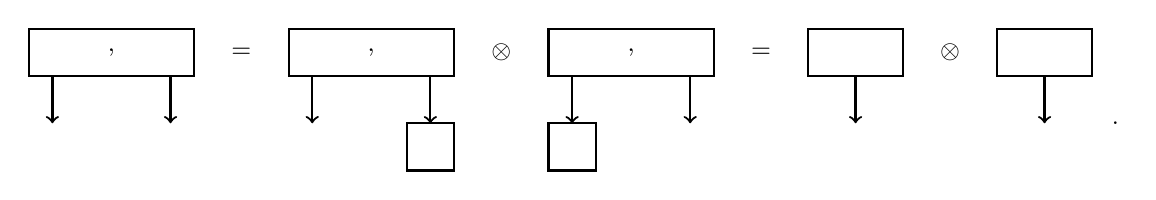
\begin{tikzpicture}[scale=0.3,thick] % , baseline = -3.5pt


\draw (0,1) rectangle (7,-1);
\node[anchor=center] (text) at (3.5,0) {\small $\probof{\exrandom,\secexrandom}$};
\draw[->] (1,-1) -- (1,-3) node[midway, left] {\tiny $\exrandom$};
\draw[->] (6,-1) -- (6,-3) node[midway, left] {\tiny $\secexrandom$};

\node[anchor=center] (text) at (9,0) {\small ${=}$};


\begin{scope}[shift={(11,0)}]

\draw (0,1) rectangle (7,-1);
\node[anchor=center] (text) at (3.5,0) {\small $\probof{\exrandom,\secexrandom}$};
\draw[->] (1,-1) -- (1,-3) node[midway, left] {\tiny $\exrandom$};
\draw[->] (6,-1) -- (6,-3) node[midway, left] {\tiny $\secexrandom$};
\draw (5,-3) rectangle (7,-5);
\node[anchor=center] (text) at (6,-4) {\small $\ones$};

\end{scope}

\node[anchor=center] (text) at (20,0) {\small $\otimes$};

\begin{scope}[shift={(22,0)}]

\draw (0,1) rectangle (7,-1);
\node[anchor=center] (text) at (3.5,0) {\small $\probof{\exrandom,\secexrandom}$};
\draw[->] (1,-1) -- (1,-3) node[midway, left] {\tiny $\exrandom$};
\draw (0,-3) rectangle (2,-5);
\node[anchor=center] (text) at (1,-4) {\small $\ones$};
\draw[->] (6,-1) -- (6,-3) node[midway, left] {\tiny $\secexrandom$};

\end{scope}

\node[anchor=center] (text) at (31,0) {\small ${=}$};

\begin{scope}[shift={(33,0)}]

\draw (0,1) rectangle (4,-1);
\node[anchor=center] (text) at (2,0) {\small $\margprobof{\exrandom}{\exrandom}$};
\draw[->] (2,-1) -- (2,-3) node[midway, left] {\tiny $\exrandom$};

\node[anchor=center] (text) at (6,0) {\small $\otimes$};

\draw (8,1) rectangle (12,-1);
\node[anchor=center] (text) at (10,0) {\small $\margprobof{\secexrandom}{\secexrandom}$};
\draw[->] (10,-1) -- (10,-3) node[midway, left] {\tiny $\secexrandom$};


\end{scope}

\node[anchor=center] (text) at (46,-3) {\small ${.}$};

\end{tikzpicture} 
	\end{center}

Independence is a very strong assumption, which is often too restrictive.
Conditional independence instead is a less demanding assumption, when certain conditional distribution variables are independent. 
This leads to tensor network decompositions with a more realistic assumption.

\begin{definition}[Conditional Independence]\label{def:condIndependence}
	Given a joint distribution of variables $\exrandom$, $\secexrandom$ and $\thirdexrandom$, we say $\exrandom$ is independent from $\secexrandom$ conditioned on $\thirdexrandom$ if for any incides $\exrandind,\secexrandind$ and $\thirdexrandind$
		\[ \condprobof{\exrandom=\exrandind,\secexrandom=\secexrandind}{\thirdexrandom=\thirdexrandind} 
		= \condprobof{\exrandom=\exrandind}{\thirdexrandom=\thirdexrandind} 
		\cdot \condprobof{\secexrandom=\secexrandind}{\thirdexrandom=\thirdexrandind}   \, . \]
\end{definition}

Conditional independence is a relation between conditional probabilities and is therefore equivalent to a normation equation stated next.

\begin{theorem}[Conditional Independence as a Contraction Equation]\label{the:condIndependenceProductCriterion}
	Given a distribution $\probtensor$ of variables $\exrandom$, $\secexrandom$ and $\thirdexrandom$, the variable $\exrandom$ is independent from $\secexrandom$ if and only if the contraction equation
	\begin{align*}
		 \condprobof{\exrandom,\secexrandom}{\thirdexrandom} 
		 = \contractionof{\{
		 \condprobof{\exrandom}{\thirdexrandom} ,\condprobof{\secexrandom}{\thirdexrandom} 
		 \}}{\exrandom,\secexrandom,\thirdexrandom}
	\end{align*}
	holds.
\end{theorem}
\begin{proof}
	Directly by Theorem~\ref{the:conditionalContraction} used on the conditional probabilities in Definition~\ref{def:condIndependence}.
\end{proof}

We can exploit conditional independence to find tensor network decompositions of probability tensors, as we show in the next theorem.

\begin{corollary}\label{cor:secCriterionCondIndepencence}
	If and only if $\exrandom$ is independent from $\secexrandom$ conditioned on $\thirdexrandom$ the probability distribution $\probtensor$ satisfies
		\[ \probof{\exrandom, \secexrandom, \thirdexrandom} 
		= \contractionof{
			\{ \condprobof{\exrandom}{\thirdexrandom}, \condprobof{\secexrandom}{\thirdexrandom}, \margprobof{\thirdexrandom}{\thirdexrandom} \}
		}{
			\exrandom, \secexrandom, \thirdexrandom
		} \, .
		\]
\end{corollary}
\begin{proof}
	Follows from Theorem~\ref{the:condIndependenceProductCriterion} and Theorem~\ref{the:bayes}.
%	We start with the chain rule decomposition of Theorem~\ref{the:chainRule} and have
%		\[ \probof{\exrandom,\secexrandom,\thirdexrandom} = \probof{\thirdexrandom}  \cdot \condprobof{\exrandom,\secexrandom}{\thirdexrandom} \]
%	Since $\exrandom$ is independent from $\secexrandom$ conditioned on $\thirdexrandom$ we have
%		\[ \condprobof{\exrandom,\secexrandom}{\thirdexrandom}  = \condprobof{\exrandom}{\thirdexrandom}  \cdot \condprobof{\secexrandom}{\thirdexrandom}  \, . \]
%	Converse direction similar.
\end{proof}


\begin{corollary}\label{cor:conditionDropping}
	Whenever $\exrandom$ is independent of $\secexrandom$ given $\thirdexrandom$, we have
	\begin{align*}
		\condprobof{\exrandom}{\secexrandom,\thirdexrandom} = \condprobof{\exrandom}{\thirdexrandom} \, .
	\end{align*}
\end{corollary}


\begin{figure}[h]
\begin{center}
	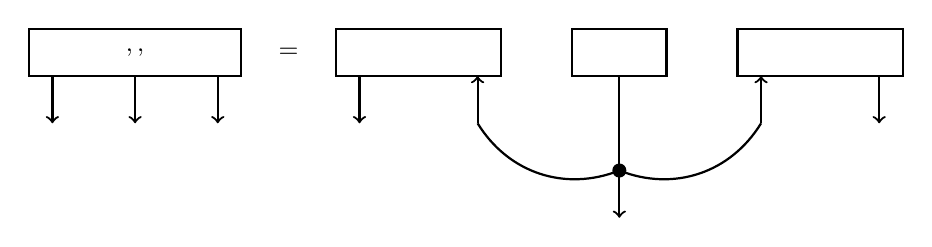
\begin{tikzpicture}[scale=0.3,thick] % , baseline = -3.5pt


\draw (-2,1) rectangle (7,-1);
\node[anchor=center] (text) at (2.5,0) {\small $\probof{\exrandom,\secexrandom,\thirdexrandom}$};
\draw[->] (-1,-1) -- (-1,-3) node[midway, left] {\tiny $\exrandom$};
\draw[->] (2.5,-1) -- (2.5,-3) node[midway, left] {\tiny $\secexrandom$};
\draw[->] (6,-1) -- (6,-3) node[midway, left] {\tiny $\thirdexrandom$};

\node[anchor=center] (text) at (9,0) {\small ${=}$};

\draw (11,1) rectangle (18,-1);
\node[anchor=center] (text) at (14.5,0) {\small $\condprobof{\exrandom}{\thirdexrandom}$};
\draw[->] (12,-1) -- (12,-3) node[midway, left] {\tiny $\exrandom$};
\draw[<-] (17,-1) -- (17,-3) node[midway, left] {\tiny $\thirdexrandom$};

\draw (21,1) rectangle (25,-1);
\node[anchor=center] (text) at (23,0) {\small $\probof{\thirdexrandom}$};
\draw (23,-1) -- (23,-3) node[midway, left] {\tiny $\thirdexrandom$};

\draw (23,-3) -- (23,-5);
\draw[fill] (23,-5) circle (0.25cm);
\draw[->] (23,-5) -- (23,-7) node[midway, left] {\tiny $\thirdexrandom$};
\draw (17,-3) to[bend right=40] (23,-5);
\draw (29,-3) to[bend right=-40] (23,-5);


\draw (28,1) rectangle (35,-1);
\node[anchor=center] (text) at (31.5,0) {\small $\condprobof{\secexrandom}{\thirdexrandom}$};
\draw[<-] (29,-1) -- (29,-3) node[midway, left] {\tiny $\thirdexrandom$};
\draw[->] (34,-1) -- (34,-3) node[midway, left] {\tiny $\secexrandom$};



\end{tikzpicture} 
\end{center}
\caption{Diagrammatic visualization of the contraction equation in Corollary~\ref{cor:secCriterionCondIndepencence}. Conditional independence of $\exrandom$ and $\secexrandom$ given $\thirdexrandom$ holds if the contraction on the right ride is equal to the probability tensor on the left side.}
\end{figure}



% More of an example?
\begin{theorem}[Markov Chain]\label{the:MarkovChain}
	Let there be a set of variables $\catvariableof{\tenumerator}$ where $\tenumeratorin$.
	When $\catvariableof{\tenumerator}$ is independent of $\catvariableof{0:{\tenumerator-2}}$ conditioned on $\catvariableof{\tenumerator-1}$ (the Markov Property), then
	\begin{align*}
		\probtensor = \contractionof{\{ \condprobof{\catvariableof{\tenumerator}}{\catvariableof{\tenumerator-1}}\, : \, \tenumeratorin \}}{
		\catvariableof{0},\ldots,\catvariableof{\tdim-1}
		} 
	\end{align*}	
%		\[ \probof{\catvariableof{0},\ldots,\catvariableof{\tdim-1}} = %\probof{\catvariableof{1}} 
%		\prod_{\tenumeratorin} \condprobof{\catvariableof{\tenumerator}}{\catvariableof{\tenumerator-1}} \, . \] 
	We depict this decomposition in Figure~\ref{fig:MC}.
\end{theorem}
\begin{proof}
	By the chain rule (Theorem~\ref{the:chainRule}) we have
	\begin{align*}
	 	\probof{\catvariableof{0},\ldots,\catvariableof{\tdim-1}}
		= \contractionof{
		\{ \condprobof{\catvariableof{\tenumerator}}{\catvariableof{0:\tenumerator}} : \tenumeratorin \}
		}{\catvariableof{[\tdim]}}
		%= \contractionof{\{\probof{\catvariableof{0}} \prod_{\tenumeratorin, \tenumerator>1} \condprobof{\catvariableof{\tenumerator}}{\catvariableof{0:\tenumerator}}\}{\catvariableof{[\tdim]}} \, . 
	\end{align*}
	Using the conditional independence of $\catvariableof{\tenumerator}$ and $\catvariableof{0:{\tenumerator-2}}$ conditioned on $\catvariableof{\tenumerator-1}$ we further have by Corollary~\ref{cor:conditionDropping}
		\[ \condprobof{\catvariableof{\tenumerator}}{\indexedcatvariableof{0:\tenumerator}}  = \condprobof{\catvariableof{\tenumerator}}{\indexedcatvariableof{\tenumerator-1}} \, .  \]
	Composing both equalities shows the claim.
\end{proof}

Here we denoted by $\catvariableof{0:\tenumerator}$ the tuple $\catvariableof{0},...,\catvariableof{\tenumerator}$.

\begin{remark}
	Let us notice that the dimensionality dropped drastically through applying the independence assumption.
	The tensor space in the naive representation of any probability distribution has
		\[ \prod_{\tenumeratorin} \catdimof{\tenumerator}\]
	coordinates, while the Markov Chain is represented by
		\[ \sum_{\tenumeratorin}  \catdimof{\tenumerator}\cdot \catdimof{\tenumerator-1} \, . \]
	Replacing exponential scaling with the number of variables to linear scaling is the advantage of tensor network decompositions.
\end{remark}

\begin{figure}[h]
\begin{center}
	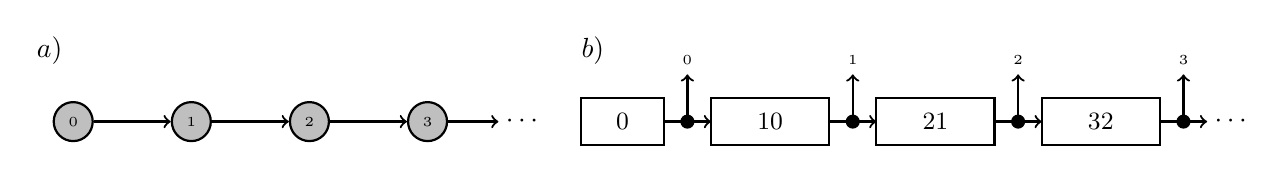
\begin{tikzpicture}[scale=0.3,thick] % , baseline = -3.5pt

\node[anchor=center] (text) at (-1,3) {${a)}$};

	\node [circle, draw, thick, fill=gray!50] (T1) at (0,0) {\tiny $\randomxof{0}$};
	\node [circle, draw, thick, fill=gray!50] (T2) at (5,0) {\tiny $\randomxof{1}$};
	\draw[->] (T1) -- (T2);
	\node [circle, draw, thick, fill=gray!50] (T3) at (10,0) {\tiny $\randomxof{2}$};
	\draw[->] (T2) -- (T3);
	\node [circle, draw, thick, fill=gray!50] (T4) at (15,0) {\tiny $\randomxof{3}$};
	\draw[->] (T3) -- (T4);
	\draw[->] (T4) -- (18,0);

	\node[anchor=center] (text) at (19,0) {$\cdots$};

	%\node [circle, draw, thick, fill=gray!50] (T4) at (17,0) {\tiny $\randomxof{\atomorder}$};
	%\draw[->] (14,0) -- (T4);	
			

\begin{scope}[shift={(25,0)}]

\node[anchor=center] (text) at (-3,3) {${b)}$};

\draw (-3.5,-1) rectangle (0, 1);
\node[anchor=center] (text) at (-1.75,0) {\small $\probof{\randomxof{0}}$};
\draw[->] (0,0) -- (2,0);
\draw[fill] (1,0) circle (0.25cm);
\draw[->] (1,0) -- (1,2) node[above] {\tiny $\catlegof{0}$};
\draw (2,-1) rectangle (7, 1);
\node[anchor=center] (text) at (4.5,0) {\small $\condprobof{\randomxof{1}}{\randomxof{0}}$};
\draw[->]  (7,0) -- (9,0);
\draw[fill] (8,0) circle (0.25cm);
\draw[->] (8,0) -- (8,2) node[above] {\tiny $\catlegof{1}$};
\draw (9,-1) rectangle (14, 1);
\node[anchor=center] (text) at (11.5,0) {\small $\condprobof{\randomxof{2}}{\randomxof{1}}$};
\draw[->]  (14,0) -- (16,0);
\draw[fill] (15,0) circle (0.25cm);
\draw[->] (15,0) -- (15,2) node[above] {\tiny $\catlegof{2}$};
\draw (16,-1) rectangle (21, 1);
\node[anchor=center] (text) at (18.5,0) {\small $\condprobof{\randomxof{3}}{\randomxof{2}}$};
\draw[->]  (21,0) -- (23,0);
\draw[fill] (22,0) circle (0.25cm);
\draw[->] (22,0) -- (22,2) node[above] {\tiny $\catlegof{3}$};
\node[anchor=center] (text) at (24,0) {$\cdots$};


\end{scope}

\end{tikzpicture} 
\end{center}
\caption{Depiction of a Markov Chain. 
	a) Dependency Graph (of the corresponding chain Graphical Model).
	b) Dual Tensor Network representing the conditional probability factors.}
\label{fig:MC}
\end{figure}





\subsection{Graphical Models}



We have already depicted conditional dependency assumptions made for Markov Chains in Figure~\ref{fig:MC} and discussed the implied decomposition of the dual tensor networks.
Graphical models provide a more general framework for conditional dependency assumptions and provide a generic approach to exploit independences in finding tensor network decompositions of $\probtensor$.

Graphical Models are typically depictured by nodes to each variable and edges.
Whether the graph is directed or not distinguished between Bayesian Networks and Markov Networks.


\begin{remark}[Alternative definitions]
	In the literature, tensor networks are often called dual to the hypergraphs defining graphical models (see e.g. \cite{robeva_duality_2019}).
	The duality becomes clear, when one interpretes the tensors as cores and their common variables as edges.
	We in this work avoid this ambiguity by directly defining tensor networks as decoration of hyperedges by tensors.
	
	Often, the tensors decorating hyperedges are called factors and their logarithm features.
	
	Further, we directly use hypergraphs instead of the more canonical association of factors with cliques of a graph.
	This avoids the discussion of non-maximal cliques as decorated with trivial tensors.
	Such hypergraphs follow the same line of though compared with factor graphs, which are bipartite graphs with nodes either corresponding with single variables or with a collection of them affected by a factor.
\end{remark}


%\begin{remark}[Further nomenclature]
%	The factors of the graphical models are tensors (since multivariate functions of discrete variables).
%	The edges are associated to each axis of the tensor and carry the variables.
%	Since each edge variable can appear in multiple factors, the Tensor Network is defined on a Hypergraph, where edges are interpreted as Hadamard contractions.
%\end{remark}

\subsubsection{Bayesian Networks}

Bayesian networks are described by directed acyclic graphs (DAG).
The probability distribution is a Hadamard product of conditional probabilities, where each variable has a conditional probability factor conditioned on the parents variables in the graph.

We introduce Bayesian Networks based on directed hypergraphs (see Definition~\ref{def:hypergraphs}) and define further properties.

\begin{definition}
%% Already in notation chapter 
%	A directed hypergraph is a tuple $\graph=(\nodes,\edges)$ of nodes $\nodes$ and hyperedges $\edges$, where each hyperedge $\edge\in\edges$ is a tuple
%		\[ \edge = (\incomingnodes,\outgoingnodes) \]
%	of disjoint sets of incoming nodes $\incomingnodes\subset\nodes$ and outgoing nodes $\outgoingnodes\subset\nodes$.
	A directed path is a sequence $\node_{0},\ldots\node_{\secatomorder}$ such that for any $\secatomenumeratorin$ there is an hyperedge $\edge=(\incomingnodes,\outgoingnodes)\in\edges$ such that $\node_{\secatomenumerator}\in\incomingnodes$ and $\node_{\secatomenumerator+1}\in\outgoingnodes$.
	We call the hypergraph $\graph$ acyclic, if there is no path with $\secatomorder>0$ such that $\node_{0}=\node_{\secatomorder}$.
	Given a directed hypergraph $\graph=(\nodes,\edges)$ we define for any node $\nodein$ its parents by
		\[ \parentsof{\node} = \{\secnode \, : \, \exists\edge=(\incomingnodes,\outgoingnodes)\in\edges: \secnode\in\incomingnodes,\node\in\outgoingnodes \} \]
	and its non-descendants $\nondescendantsof{\node}$ as the set of nodes $\secnode$, such that there is no directed path from $\node$ to $\secnode$.
\end{definition}

\begin{definition}
	%Let $\nodes$ be a set of nodes decorated by dimensions and 
	Let $\graph=(\nodes,\edges)$ be a directed acyclic hypergraph with edges of the form 
		\[ \edges = \{(\parentsof{\node},\{\node\}) \, : \, \nodein\} \, . \]
%	and for each node $\node\in\nodes$ a random variable $\catvariableof{\node}$.
	A \emph{Bayesian Network} is a decoration of each edge $(\parentsof{\node},\{\node\})$ by a conditional probability distribution
	%Further let there be for each node $\node\in\nodes$ with parents $\parentsof{\node}$ a conditional probability distribution
		\[ \condprobof{\catvariableof{\node}}{\catvariableof{\parentsof{\node}}} \]
	which represents the probability distribution
%	Then the \emph{Bayesian Network} with respect to $\graph$ and the conditional probability terms is the distribution
	\begin{align*}
		\probof{\nodevariables} = \contractionof{\{\condprobof{\catvariableof{\node}}{\catvariableof{\parentsof{\node}}} \, : \, \nodein\}}{\nodevariables} \, .
	\end{align*}
%		\[ \probof{\catvariableof{\node} \, : \, \node\in\nodes } = \prod_{\node\in\nodes} \condprobof{\catvariableof{\node}}{\catvariableof{\parentsof{\node}}} \, . \]
\end{definition}

%
By definition each tensor decorating a hyperedge is directed with $\catvariableof{\parentsof{\node}}$ incoming and $\catvariableof{\node}$ outgoing.
Thus, the directionality of the hypergraph is reflected in each tensor decorating a directed hyperedge.
This allows us to verify with Theorem~\ref{the:conditionalContractionPreservation} that their contraction defines a probability distribution.

% Contraction -> Now in definition!
%By definition we can represent a Bayesian network by the contraction
%\begin{align*}
%	\probtensorof{\graph} = \sbcontractionof{\{ \condprobof{\catvariableof{\node}}{\catvariableof{\parentsof{\node}}} \, : \, \node\in\nodes\}}{\nodes} \, . 
%\end{align*}

% Dual
%The dual tensor network consists of conditional probability distributions to each node $\node\in\nodes$ (see Figure~\ref{fig:BayesianFactor}b).

\begin{figure}[h]
\begin{center}
	\begin{tikzpicture}[scale=0.35,thick] % , baseline = -3.5pt

\node[anchor=center] (text) at (-1,3) {${a)}$};

	\node [circle, draw, thick, fill=gray!50] (H) at (5,0) {\tiny $\randomxof{\node}$};
	\node [circle, draw, thick, fill=gray!50] (P1) at (0,-5) {\tiny $\randomxof{0}$};	
	\node [circle, draw, thick, fill=gray!50] (P2) at (5,-5) {\tiny $\randomxof{1}$};	
	
	\node[anchor=center] (text) at (10,-5) {$\cdots$};
	\node [circle, draw, thick, fill=gray!50] (Pd) at (15,-5) {\tiny $\randomxof{\atomorder\shortminus1}$};
	
	\node [] (E) at (5,-2) {};	
	
	\draw[midarrow] (P1) -- (5,-2) ;	
	\draw[midarrow] (P2) -- (5,-2) ;	
	\draw[midarrow] (Pd) -- (5,-2) ;	
	\draw[midarrow] (5,-2) -- (H) ;	
			

\begin{scope}[shift={(25,0)}]

\node[anchor=center] (text) at (-3,3) {${b)}$};

\draw[->] (4.5,-1) -- (4.5,1) node[midway, right]{\tiny $\catvariableof{\node}$};
\draw (0,-1) rectangle (9,-4); 
\node[anchor=center] (text) at (4.5,-2.5) {\small $\condprobof{\randomxof{\node}}{\randomxof{[\atomorder]}} $};
\draw[->] (1,-6) -- (1,-4) node[midway, right]{\tiny $\catlegof{0}$};
\draw[->] (2.5,-6) -- (2.5,-4) node[midway, right]{\tiny $\catlegof{1}$};

\node[anchor=center] (text) at (5.5,-5) {$\cdots$};
	
\draw[->] (8,-6) -- (8,-4) node[midway, right]{\tiny $\catlegof{\atomorder\shortminus1}$};

\end{scope}

\end{tikzpicture} 
\end{center}
\caption{Example of a Factor of a Bayesian Network to the node $\catvariableof{\node}$ with parents $\catvariableof{0},\ldots,\catvariableof{\catorder-1}$, as subgraph $a)$ and dual tensor core $b)$.}
\label{fig:BayesianFactor}
\end{figure}


%% Marginalization and Contraction
Marginalization of a Bayesian Network are still Bayesian Networks on a graph where the edges directing to variables, which are not marginalized over, are replaced by directed edges to the children.
Conditioned Bayesian Network do not have a simple Bayesian Network representation, which is why we will treat them as Markov Networks to be introduced next.


\begin{theorem}[Independence Characterization of Bayesian Networks]\label{the:condIndBN}
	A probability distribution $\probof{\nodevariables}$ has a representation by a Bayesian Network on a directed acyclic graph $\graph=(\nodes,\edges)$, if and only if for any $\nodein$ the variables $\catvariableof{\node}$ are independent on $\nondescendantsof{\node}$ conditioned on $\parentsof{\node}$.
\end{theorem}
\begin{proof}
	We choose a topological order $\prec$ on the nodes of $\graph$, which exists since $\graph$ is acyclic.
	% =>
	Let us assume, that the conditional independencies are satisfied and apply the chain rule with respect to that ordering to get
	\begin{align*}
		\probof{\nodevariables} =
		\contractionof{
			\condprobof{\catvariableof{\node}}{\catvariableof{\secnode} : \secnode \prec \node}
		}
		{\nodevariables} \, .
	\end{align*}
	Since $\prec$ is a topological ordering we have
		\[ \parentsof{\node} \subset \{\secnode : \secnode \prec \node\} \]
	We apply the assumed conditional independence with Corollary~\ref{cor:conditionDropping} and get
	\begin{align*}
		\probof{\nodevariables} =
		\contractionof{
			\condprobof{\catvariableof{\node}}{\catvariableof{\parentsof{\node}}}
		}
		{\nodevariables} \, .
	\end{align*}
	% <=
	To show the converse direction, let there be a Bayesian Network $\probof{\nodevariables}$ on $\graph$.
	To show for any node $\node$, that $\catvariableof{\node}$ is independent of $\nondescendantsof{\node}$ conditioned on $\parentsof{\node}$, we reorder the tensors in the contraction
	%with respect to a set $\node_0$ 
	\begin{align*}
		\condprobof{\catvariableof{\node},\catvariableof{\nondescendantsof{\node}}}{\indexedcatvariableof{\parentsof{\node}}}
		& = \normationofwrt{
			\{\condprobof{\catvariableof{\secnode}}{\parentsof{\secnode}} \, : \, \secnode\in\nodes\}
		}
		{\catvariableof{\node},\catvariableof{\nondescendantsof{\node}}}
		{\indexedcatvariableof{\parentsof{\node}}} \\
		& = \normationof{
			\{\condprobof{\catvariableof{\secnode}}{\parentsof{\secnode}} \, : \, \secnode\in\nodes\} \cup \{\onehotmapof{\catindexof{\parentsof{\node}}}\}
		}
		{\catvariableof{\node},\catvariableof{\nondescendantsof{\node}}}\\
		& = \normationof{
			\{\condprobof{\catvariableof{\secnode}}{\parentsof{\secnode}} \, : \, \secnode\in\nondescendantsof{\node}\} \cup \{\onehotmapof{\catindexof{\parentsof{\node}}}, \condprobof{\catvariableof{\node}}{\parentsof{\node}} \}
		}
		{\catvariableof{\node},\catvariableof{\nondescendantsof{\node}}} \\
		& =  %\contractionof{
		 \normationof{
			\{\condprobof{\catvariableof{\secnode}}{\parentsof{\secnode}} \, : \, \secnode\in\nondescendantsof{\node}\} \cup \{\onehotmapof{\catindexof{\parentsof{\node}}}\}
		}
		{\catvariableof{\nondescendantsof{\node}}} \\
		& \quad  \cdot \normationof{
			\{\condprobof{\catvariableof{\node}}{\parentsof{\node}},\onehotmapof{\catindexof{\parentsof{\node}}}\}
		}
		{\catvariableof{\node}} \\
		& = \contractionof{\{
		\condprobof{\catvariableof{\nondescendantsof{\node}}}{\indexedcatvariableof{\parentsof{\node}}},
		\condprobof{\catvariableof{\node}}{\indexedcatvariableof{\parentsof{\node}}}
		\}}{\catvariableof{\node},\catvariableof{\nondescendantsof{\node}}}
		%}{\catvariableof{\node},\catvariableof{\nondescendantsof{\node}}}
	\end{align*}
	Here we have dropped in the third equation all tensors to the descendants, since their marginalization is trivial (which can be shown by a leaf-stripping argument).
	In the fourth equation we made use of the fact, that any directed path between the non-descendants and the node is through the parents of the node.
	By Theorem~\ref{the:condIndependenceProductCriterion}, it now follows that $\catvariableof{\node}$ is independent of $\nondescendantsof{\node}$ conditioned on $\parentsof{\node}$.
\end{proof}



\subsubsection{Example of a Bayesian Network: Hidden Markov Models}

We here extend the example of Markov Chains from Theorem \ref{the:MarkovChain} to a limited observation of the variables by observations.
Let there be the variables $\catvariableof{\tenumerator}$ (states) and $\randomeof{\tenumerator}$ (observations) with a discrete and finite time $\tenumeratorin$.

The conditional assumptions are 
\begin{itemize}
	\item $\catvariableof{\tenumerator+1}$ is independent of $\catvariableof{0:\tenumerator-1}$ and $\randomeof{0:\tenumerator}$ conditioned on $\catvariableof{\tenumerator}$
	\item $\randomeof{\tenumerator}$ is independent of all other variables conditioned on $\catvariableof{\tenumerator}$
\end{itemize}

Then the probability tensor has the decomposition 
\begin{align}
	\probof{\catvariableof{0:\tdim},\randomeof{0:\tdim}} 
	& = \prod_{\tenumeratorin}
	 \left( \condprobof{\catvariableof{\tenumerator}}{\catvariableof{0:\tenumerator-1},\randomeof{0:\tenumerator-1}} \cdot \condprobof{\randomeof{\tenumerator}}{\catvariableof{0:\tenumerator},\randomeof{0:\tenumerator-1}} \right) \\
	& = \probof{\catvariableof{0}} \cdot \condprobof{\randomeof{0}}{\catvariableof{0}} \cdot \prod_{\tenumeratorin, \tenumerator>0} 
	\left( \condprobof{\catvariableof{\tenumerator}}{\catvariableof{\tenumerator-1}} \cdot \condprobof{\randomeof{\tenumerator}}{\catvariableof{\tenumerator}} \right)
\end{align}
Here we used the Chain Rule decomposition of Theorem~\ref{the:chainRule} in the first equation and the conditional independence assumptions in the second.

We notice, that this is a Bayesian Netowork on a directed acyclic hypergraph $\graph$ consistent in nodes to each state and each observation and hyperedges
\begin{itemize}
	\item $(\{\catvariableof{\tenumerator}\}, \{\catvariableof{\tenumerator+1}\})$ for $\tenumerator\in[\tdim-1]$
	\item $(\{\catvariableof{\tenumerator}\}, \{\randomeof{\tenumerator}\})$ for $\tenumeratorin$
\end{itemize}


\begin{figure}[h]
\begin{center}
	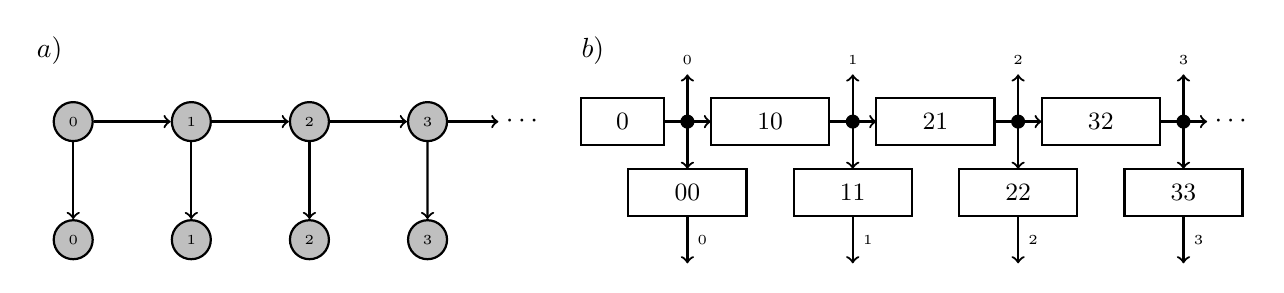
\begin{tikzpicture}[scale=0.3,thick] % , baseline = -3.5pt

\node[anchor=center] (text) at (-1,3) {${a)}$};

	\node [circle, draw, thick, fill=gray!50] (T1) at (0,0) {\tiny $\randomxof{0}$};	
	\node [circle, draw, thick, fill=gray!50] (E1) at (0,-5) {\tiny $\randomeof{0}$};
	\draw[->] (T1) -- (E1);	
	\node [circle, draw, thick, fill=gray!50] (T2) at (5,0) {\tiny $\randomxof{1}$};
	\node [circle, draw, thick, fill=gray!50] (E2) at (5,-5) {\tiny $\randomeof{1}$};
	\draw[->] (T2) -- (E2);	
	\draw[->] (T1) -- (T2);	
	\node [circle, draw, thick, fill=gray!50] (T3) at (10,0) {\tiny $\randomxof{2}$};
	\node [circle, draw, thick, fill=gray!50] (E3) at (10,-5) {\tiny $\randomeof{2}$};
	\draw[->] (T3) -- (E3);	
	\draw[->] (T2) -- (T3);
	\node [circle, draw, thick, fill=gray!50] (T4) at (15,0) {\tiny $\randomxof{3}$};
	\node [circle, draw, thick, fill=gray!50] (E4) at (15,-5) {\tiny $\randomeof{3}$};
	\draw[->] (T4) -- (E4);	
	\draw[->] (T3) -- (T4);
	\draw[->] (T4) -- (18,0);

	\node[anchor=center] (text) at (19,0) {$\cdots$};

	%\node [circle, draw, thick, fill=gray!50] (T4) at (17,0) {\tiny $\randomxof{\atomorder}$};
	%\draw[->] (14,0) -- (T4);	
			

\begin{scope}[shift={(25,0)}]

\node[anchor=center] (text) at (-3,3) {${b)}$};

\draw (-3.5,-1) rectangle (0, 1);
\node[anchor=center] (text) at (-1.75,0) {\small $\probof{\randomxof{0}}$};
\draw[->] (0,0) -- (2,0);
\draw[fill] (1,0) circle (0.25cm);
\draw[->] (1,0) -- (1,2) node[above] {\tiny ${\randomxof{0}}$};
\draw[->] (1,0) -- (1,-2);
\draw (-1.5,-2) rectangle (3.5,-4); 
\node[anchor=center] (text) at (1,-3) {\small $\condprobof{\randomeof{0}}{\randomxof{0}}$};
\draw[->] (1,-4) -- (1,-6) node[midway, right]{\tiny ${\randomeof{0}}$};

\draw (2,-1) rectangle (7, 1);
\node[anchor=center] (text) at (4.5,0) {\small $\condprobof{\randomxof{1}}{\randomxof{0}}$};
\draw[->]  (7,0) -- (9,0);
\draw[fill] (8,0) circle (0.25cm);
\draw[->] (8,0) -- (8,2) node[above] {\tiny ${\randomxof{1}}$};
\draw[->] (8,0) -- (8,-2);
\draw (5.5,-2) rectangle (10.5,-4); 
\node[anchor=center] (text) at (8,-3) {\small $\condprobof{\randomeof{1}}{\randomxof{1}}$};
\draw[->] (8,-4) -- (8,-6) node[midway, right]{\tiny ${\randomeof{1}}$};


\draw (9,-1) rectangle (14, 1);
\node[anchor=center] (text) at (11.5,0) {\small $\condprobof{\randomxof{2}}{\randomxof{1}}$};
\draw[->]  (14,0) -- (16,0);
\draw[fill] (15,0) circle (0.25cm);
\draw[->] (15,0) -- (15,2) node[above] {\tiny ${\randomxof{2}}$};
\draw[->] (15,0) -- (15,-2);
\draw (12.5,-2) rectangle (17.5,-4); 
\node[anchor=center] (text) at (15,-3) {\small $\condprobof{\randomeof{2}}{\randomxof{2}}$};
\draw[->] (15,-4) -- (15,-6) node[midway, right]{\tiny ${\randomeof{2}}$};

\draw (16,-1) rectangle (21, 1);
\node[anchor=center] (text) at (18.5,0) {\small $\condprobof{\randomxof{3}}{\randomxof{2}}$};
\draw[->]  (21,0) -- (23,0);
\draw[fill] (22,0) circle (0.25cm);
\draw[->] (22,0) -- (22,2) node[above] {\tiny ${\randomxof{3}}$};
\draw[->] (22,0) -- (22,-2);
\draw (19.5,-2) rectangle (24.5,-4); 
\node[anchor=center] (text) at (22,-3) {\small $\condprobof{\randomeof{3}}{\randomxof{3}}$};
\draw[->] (22,-4) -- (22,-6) node[midway, right]{\tiny ${\randomeof{3}}$};


\node[anchor=center] (text) at (24,0) {$\cdots$};


\end{scope}

\end{tikzpicture} 
\end{center}
\caption{Depiction of a Hidden Markov Model. 
	a) Dependency Graph (of the corresponding chain Graphical Model).
	b) Dual Tensor Network representing the conditional probability factors.}
\label{fig:HMM}
\end{figure}



\subsubsection{Markov Networks}

\red{While typically Markov Networks are defined on graphs, we define them here on hypergraphs to establish a direct connection to tensor networks defined on the same hypergraph.}
Along that line, Markov Networks are tensor networks with non-negative tensors (see Definition~\ref{def:tensorNetwork}), which are interpreted as probability distributions after normation.

\begin{definition}\label{def:markovNetwork}
	Let $\tnetof{\graph}$ be a Tensor Network on a hypergraph $\graph$.
	Then the Markov Network to $\tnetof{\graph}$ is the probability distribution of $\catvariableof{\node}$ defined by the tensor
		\[ \probtensorof{\graph} = \frac{
			\contractionof{\{\hypercoreof{\edge} : \edge \in \edges\}}{\nodes} 
		}{
			\contraction{\{\hypercoreof{\edge} : \edge \in \edges\}}
		} = \normationof{\{\hypercoreof{\edge} : \edge \in \edges\}}{\nodes} \, . \] 
	We call the denominator
		\[\partitionfunctionof{\graph} = \contraction{\{\hypercoreof{\edge} : \edge \in \edges\}} \]
	the partition function of the Markov Network.
\end{definition}

%
This established a generic relation between Markov Networks and Tensor Networks with coordinatewise non-negative contractions.

%


% Marginalization and Conditioning
Let us now demonstrate how marginalizations and contractions can be done on Markov Networks.

\begin{theorem}[Marginalization by Contractions]
	The marginalization of a Markov Network to $\tnetof{\graph}$ on the variables of the subset $\secnodes$ is
	\[
		\probtensor^{\graph}\left[ \catvariableof{\secnodes}\right] 
		= \contractionof{\tnetof{\graph}}{\catvariableof{\secnodes}}
	\]
	and the distribution of $\secnodes$ conditioned on $\thirdnodes$ is
	\[
		\probtensor^{\graph}\left[ \catvariableof{\secnodes} | \catvariableof{\thirdnodes}\right] 
		= \normationofwrt{\tnetof{\graph}}{\catvariableof{\secnodes}}{\catvariableof{\thirdnodes}}
	\]
\end{theorem}
\begin{proof}
	From contraction by subcontraction Theorem~\ref{the:splittingContractions}.
\end{proof}

%Markov networks are especially good at incorporating evidence.
%Bayesian networks on the other side always need to impose local normation conditions, which drop when conditioning on evidence.

%\begin{theorem}
%	The Markov Network conditioned on evidence is the Markov Network, where the evidence is added as decoration of an additional hyperedge.
%\end{theorem}

\begin{definition}[Separation of Hypergraph]
	A path in a hypergraph is a sequence of nodes $\node_{\atomenumerator}$ for $\atomenumeratorin$, such that for any $\atomenumerator\in[\atomorder-1]$ we find a hyperedge $\edge\in\edges$ such that $(\node_{\atomenumerator}, \node_{\atomenumerator+1})\subset \edge$.
	Given disjoint subsets $\nodesa$, $\nodesb$, $\nodesc$ of nodes in a hypergraph $\graph$ we say that $\nodesc$ separates $\nodesa$ and $\nodesb$ with respect to $\graph$, when any path starting at a node in $\nodesa$ and ending in a node in $\nodesb$ contains a node in $\nodesc$.
	%when removing the hyperedges which are contained in $\nodesc$ leads to a hypergraph with no path of hyperedges between a node in $\nodesa$ to a node in $\nodesb$.
\end{definition}

To characterize Markov Networks in terms of coditional independencies we need to further define the property of clique-capturing.

\begin{definition}[Clique-Capturing Hypergraph]
	We call a hypergraph $\graph$ clique-capturing, when each subset $\secnodes\subset\nodes$ is contained in a hyperedge, if for any $a,b\in\secnodes$ there is a hyperedge $\edge\in\edges$ with $a,b\in\secnodes$.
\end{definition}

Let us now show a characterization of Markov Networks in terms of conditional independencies, which is analogous to Theorem~\ref{the:condIndBN}.

% Characterization
\begin{theorem}\label{the:condIndMN}
	Given a clique-capturing hypergraph $\graph$, the set of positive Markov Networks on the hypergraph coincides with the set of positive probability distributions, such that each for each disjoint subsets of variables $\nodesa$, $\nodesb$, $\nodesc$ we have $\catvariableof{\nodesa}$ is independent of $\catvariableof{\nodesb}$ conditioned on $\catvariableof{\nodesc}$, when $\nodesc$ separates $\nodesa$ and $\nodesb$ in the hypergraph. % called d-separation
\end{theorem}
\begin{proof}
	%=>
	%Given any Markov Network, contracting with $\onehotmapof{\atomlegindexof{\nodesc}}$ turns all hyperedges contained in $\nodesc$ to scalar factors (copying possible).
	Let there be a hypergraph $\graph$, a Markov Network $\extnet$ on $\graph$ and nodes $\nodesa,\nodesb,\nodesc \subset \nodes$, such that $\nodesc$ separates $\nodesa$ from $\nodesb$.
	Let us denote by $\nodes_0$ the nodes with paths to $\nodesa$, which do not contain a node in $\nodesc$, and by $\nodes_1$ the nodes with paths to $\nodesb$, which do not contain a node in $\nodesc$.
	Further, we denote by $\edges_0$ the hyperedges which contain a node in $\nodes_0$ and by $\edges_1$ the hyperedges which contain a node in $\nodes_1$.
	By assumption of separability, both sets $\edges_0$ and $\edges_1$ are disjoint and no node in $\nodesa$ is in a hyperedge in $\edges_1$, respectively no node in $\nodesb$ is in a hyperedge in $\edges_0$, .
	We then have
	\begin{align*}
		\normationofwrt{\extnetasset}{\catvariableof{\nodesa},\catvariableof{\nodesb}}{\indexedcatvariableof{\nodesc}} 
		= & \normationof{\extnetasset\cup\{\onehotmapof{\catindexof{\nodesc}}\}}{\catvariableof{\nodesa},\catvariableof{\nodesb}} \\
		= &  \normationof{\{\hypercoreof{\edge}\, : \, \edge\in\edges_0\}\cup\{\onehotmapof{\catindexof{\nodesc}}\}}{\catvariableof{\nodesa}}
		\otimes \normationof{\{\hypercoreof{\edge}\, : \, \edge\in\edges_1\}\cup\{\onehotmapof{\catindexof{\nodesc}}\}}{\catvariableof{\nodesb}} \, .
	\end{align*}
	By Theorem~\ref{the:condIndependenceProductCriterion}, it now follows that $\catvariableof{\nodesa}$ is independent of $\catvariableof{\nodesb}$ conditioned on $\catvariableof{\nodesc}$.
	%<= HARDER! Hammersley Clifford needed
	The converse direction, i.e. that positive distributions respecting the conditional indpendence assumptions are representable as Markov Networks, is known as the Hammersley Clifford Theorem, 
	which we will proof later in Section~\ref{sec:proofHCTheorem}.
	%for which proof we refer to Theorem~4.8 in KOLLER.
\end{proof}

% Positivity
From the proof of Theorem~\ref{the:condIndMN} Markov Networks with zero coordinates still satisfy the conditional independence assumption.
However, the reverse is not true, that is there are distributions with vanishing coordinates, which satisfy the conditional independence assumptions, but cannot be represented as a Markov Network (see Example~4.4 in \cite{koller_probabilistic_2009}).

\subsubsection{Bayesian Networks as Markov Networks}

Markov Networks are more flexible compared with Bayesian Networks, since any Bayesian Network is a Markov Network, as we will show in the next theorem.

\begin{theorem}\label{the:BayesianToMarkov}
	Any Bayesian Network on a directed graph $\graph=(\nodes,\edges)$ is a Markov Network on a hypergraph $\secgraph=(\nodes,\secedges)$ with identical nodes and hyperedges consistent of  a hyeredge to each node with $\node$ being the only outgoing node and
		\[  \{\tilde{\node} \, : \, (\tilde{\node},\node) \in \edges\} \,  \]
	being the incoming nodes.
	Each hyperedge of the Markov Network is decorated with the conditional probability distribution and the partition function is vanishing.
\end{theorem}
\begin{proof}
	Each conditional probability distribution is associated with the hyperedge constructed to the representative node.
	The contraction of all conditional probability distributions is the Bayesian Network, which corresponds with the constructed Markov Network due to the trivial partition function.
\end{proof}

%% Bayesian Network richer
Theorem~\ref{the:BayesianToMarkov} states that Markov Networks are more generic compared with Bayesian Networks.
While Markov Network allow for any Tensor Cores and norming the probability distribution globally, Bayesian Networks impose a local normation condition on each Tensor Core by demanding it to be a conditional probability tensor.
In our diagrammatic notation, the local normation of Bayesian Networks is highlighted by the directionality of the hypergraph.
Generic Markov Networks are on undirected hypergraphs, where no local normation condition applies.

%% Conditioning
The representation of Bayesian Networks by Markov Networks is of special interest when representing conditional distributions.
Bayesian Networks conditioned on evidence are no longer Bayesian Networks on the same graph, but Markov Networks on a hypergraph enriched by the evidence conditioned about.








\subsection{Exponential Families}\label{sec:exponentialFamilies}

% Usage of the selection encoding -> Can also make a theorem out of this
Exponential families are collections of probability distributions, where each coordinate is determined by a base measure and a set $\sstat$ of features as
	\[ \probat{\indexedshortcatvariables}  \propto \basemeasure(\catindex) \cdot \expof{\sum_{\statenumeratorin} \sstatcoordinateofat{\selindex}{\indexedshortcatvariables} \cdot \canparamat{\indexedselvariable}} \, . \]
We use the selection encoding to represent the weighted summation over the statistics, that is the tensor
	\[ \sencsstatat{\shortcatvariables,\selvariable}: \facstates \times [\statorder] \rightarrow \rr \]
with
	\[ \sencsstatat{\indexedshortcatvariables,\indexedselvariable} = \sstatcoordinateofat{\selindex}{\indexedshortcatvariables} \, . \]
We then understand $\canparam$ as a vector to the categorical variable $\selvariable$ and use Theorem~\ref{the:linCompSelEncoding} to get
	\[ \sum_{\statenumeratorin}\canparamat{\indexedselvariable}\cdot \sstatcoordinateofat{\selindex}{\shortcatvariables}
		 = \sbcontractionof{\sencsstatat{\shortcatvariables,\selvariable},\canparamat{\selvariable}}{\shortcatvariables} \, . \]

\begin{definition}
	Given a sufficient statistics 
		\[ \sstat : \facstates \rightarrow \parameterspace\]
%		\[ \sstat : \atomstates \times [\statorder] \rightarrow \rr \]
	and a non-negative base measure
		\[ \basemeasure : \facstates \rightarrow \rr \]
	the set $\expfamily=\{\expdist \, : \, \canparam[\selvariable] \in \simpleparspace\}$ of probability distributions 
		\[ \expdist = \normationof{\expof{\sbcontractionof{\sencodingof{\sstat},\canparam}{\shortcatvariables}}}{\shortcatvariables} \]
	is called the exponential family to $\sstat$.
	If the base measure is positive, we define for each member with parameters $\canparam$
		\[ \expenergy = \sbcontractionof{\sencsstat,\canparam,\lnof{\basemeasure}}{\shortcatvariables} \]
	the associated energy tensor.
	We further introduce the cumulant function
		\[ \cumfunctionof{\canparam} = \lnof{\sbcontraction{\basemeasure,\expof{\sbcontractionof{\sencsstat,\canparam}{\shortcatvariables} }} } \, .\]
\end{definition}


%We have
%	\[ \expenergyat{\indexedcatvariables} = \sum_{\statenumeratorin}\sstatcoordinateof{\statenumerator}(\catindices) \cdot \canparam(\statenumerator) \, . \]

% Diverging partition functions avoided here
Since we here restrict the discussion to finite state spaces, the distribution $\expdist$ is well-defined for any $\canparam\in\rr^{\statorder}$.
For infinite state space there are sufficient statistics and parameters, such that the partition function $\sbcontraction{\basemeasure,\expof{\sbcontractionof{\sencsstat,\canparam}{\shortcatvariables}}}$ diverges and the normation $\expdist$ is not defined.
In that cases, the canonical parameters need to be chosen from a subset where the partition function is finite. 

% Cumulant representation
\begin{lemma}\label{lem:energyCumulantRepresentation}
	For any member of an exponential family $\expfamily$ with positive base measure we have
		\[ \expdist = \expof{ \expenergy - \cumfunctionof{\canparam}\cdot \onesat{\shortcatvariables}} \, . \]
\end{lemma}
\begin{proof}
	By definition we have
	\begin{align*}
		\expdist 
		&= \normationof{
		\expof{\sbcontractionof{\sencsstat,\canparam}{\shortcatvariables}}
		}{\shortcatvariables} \\
		&= \frac{\contractionof{\expof{\sbcontractionof{\sencsstat,\canparam}{\shortcatvariables}}}{\shortcatvariables}
			}{\contraction{\expof{\sbcontractionof{\sencodingof{\sstat},\canparam	}{\shortcatvariables}}}} \\
		&=  \frac{
		\contractionof{\expof{\expenergyat{\shortcatvariables}}}{\shortcatvariables}
		}{
		\expof{\cumfunctionof{\canparam}}
		} \\
		& = \expof{ \expenergyat{\shortcatvariables} - \cumfunctionof{\canparam}\cdot \onesat{\shortcatvariables}} \, . 
	\end{align*}
\end{proof}


\subsubsection{Tensor Network Representation} 

We can use the relational encoding formalism to represent members of exponential families by a single contraction, as we show next.
The central insight here is a relational encoding of the sufficient statistics, which enables representation by tensor network decomposition, when the sufficient statistic is decomposable.

\begin{theorem}[Generic Representation of Exponential Families]\label{def:expFamilyTensorRep}
	Given any base measure $\basemeasure$ sufficient statistic $\sstat$ we enumerate for each coordindate $\selindexin$ the image $\imageof{\sstatcoordinateof{\selindex}}$ by a variable $\sstatcatof{\selindex}$ taking values in $[\cardof{\imageof{\sstatcoordinateof{\statenumerator}}}]$, given an interpretation map
		\[ \indexinterpretationof{\selindex} : 
		[\cardof{\imageof{\sstatcoordinateof{\statenumerator}}}] \rightarrow \imageof{\sstatcoordinateof{\statenumerator}} \, . \]
	
	For any parameter vector $\canparamat{\selvariable}:[\seldim]\rightarrow\rr$ we build the activation cores
		\[ \headcoreofat{\statenumerator}{\sstatcatof{\selindex}=\sstatindof{\selindex}} 
		= \expof{\canparamat{\indexedselvariable} \cdot \indexinterpretationofat{\selindex}{\sstatcatof{\selindex}} } \,   \]
	and have
		\[ \expdist = 
		\normationof{\{\basemeasure,\rencodingof{\sstat}\}\cup\{\headcoreof{\statenumerator} \, : \, \statenumeratorin\}}{\shortcatvariables} \, . 
		\]
%	where we use the vectors $\headcoreof{\statenumerator} : \imageof{\sstatcoordinateof{\statenumerator}} \rightarrow \rr $ defined for $y \in \imageof{\sstatcoordinateof{\statenumerator}}$ by
\end{theorem}
\begin{proof}
	We use an extended image of $\sstat$ by  %	which does not modify the statement of Theorem~\ref{the:tensorFunctionComposition} (since extension to cases, which are never met).
		\[ \imageof{\sstat} = \bigtimes_{\statenumeratorin} \imageof{\sstatcoordinateof{\selindex}} \, . \]
	Theorem~\ref{the:tensorFunctionComposition} implies
		\[ \expof{\contractionof{\{\sstat, \canparam\}}{X}}
		= \contractionof{\{\rencodingof{\sstat}, \restrictionofto{\expof{\braket{\cdot, \weight}}}{\imageof{\sstat}} \}}{X} \, . \]
	The claim follows from the equation
		\[ \restrictionofto{\expof{\braket{\cdot, \canparam}}}{\imageof{\sstat}} 
		= \bigotimes_{\selindexin} \restrictionofto{\expof{\cdot \canparamat{\indexedselvariable}}}{\imageof{\sstatcoordinateof{\selindex}}}  
		= \bigotimes_{\selindexin} \headcoreof{\selindex} \, . \]
\end{proof}


We notice, that the relational encoding is the contraction of the relational encoding of its coordinate maps as 
	\[ \rencodingofat{\sstat}{\shortcatvariables,\sstatcatof{[\seldim]}} = \contractionof{\rencodingof{\sstatcoordinateof{0}},\ldots,\rencodingof{\sstatcoordinateof{\seldim-1}}}{\shortcatvariables,\sstatcatof{[\seldim]}} \, .  \]
We will show this property in Theorem~\ref{the:functionDecompositionBasisCP}.
One strategy to create $\rencodingof{\sstat}$ is thus the creation of the encoding of all its coordinate maps.
When the coordinate maps are sharing common components, a sparser representation can be derived through encodings of the components shared among the coordinate map encodings.


% Core types
A tensor network representation of an exponential family is thus a Markov Network consistent of two types of cores.
Computation cores are relational encodings of statistics $\rencodingof{\sstatcoordinateof{\selindex}}$.
Our intuition is that they compute the hidden variable $\catvariableof{\sstatcoordinateof{\selindex}}$, based on Basis Calculus (see Chapter~\ref{cha:basisCalculus}).
Activation cores $\headcoreof{\selindex}$ exploit the computed variable and provide, when contracted with the relational encoding, a factor 
	\[ \sbcontractionof{\rencodingof{\sstatcoordinateof{\selindex}}, \headcoreofat{\statenumerator}{\catvariableof{\statenumerator}}}{\shortcatvariables}  \]
to the Markov Network reduced to the visible coordinates $\shortcatvariables$.
The activation cores are trivial, i.e. $\headcoreofat{\selindex}{\sstatcatof{\selindex}}=\onesat{\sstatcatof{\selindex}}$, when $\canparamat{\selvariable=\selindex}=0$.
In that case 
	\[  \sbcontractionof{\rencodingof{\sstatcoordinateof{\selindex}}, \headcoreofat{\statenumerator}{\catvariableof{\statenumerator}}}{\shortcatvariables} 
	= \onesat{\shortcatvariables} \]
and both the activation core and the corresponding computation core can be dropped from the network without changing its distribution.

%% FALSE STATEMENT? 
%We can sum multiples of the trivial tensor on the head cores without changing the distribution as we show next.
%
%\begin{theorem}
%	For any $\statenumeratorin$, the distribution is invariant under replacing $\headcoreofat{\statenumerator}{\selvariableof{\statenumerator}}$ by $\headcoreofat{\statenumerator}{\catvariableof{\statenumerator}}+\lambda\cdot \onesat{\catvariableof{\statenumerator}}$ where $\lambda\in\rr$
%\end{theorem}
%\begin{proof}
%	Follows from linearity in each head core, trivialization by trivial heads and normation.
%	
%	By linearity we have
%	\begin{align*}
%		\sbcontractionof{\rencodingof{\sstatcoordinateof{\selindex}}, (\headcoreofat{\statenumerator}{\catvariableof{\statenumerator}}+\lambda\cdot \onesat{\catvariableof{\statenumerator}})}{\shortcatvariables}
%		= 
%		\sbcontractionof{\rencodingof{\sstatcoordinateof{\selindex}}, \headcoreofat{\statenumerator}{\catvariableof{\statenumerator}}}{\shortcatvariables}
%		+\lambda\cdot  \sbcontractionof{\rencodingof{\sstatcoordinateof{\selindex}}, \onesat{\catvariableof{\statenumerator}}}{\shortcatvariables}
%		=  \sbcontractionof{\rencodingof{\sstatcoordinateof{\selindex}}, \headcoreofat{\statenumerator}{\catvariableof{\statenumerator}}}{\shortcatvariables}
%		+ \lambda \cdot \onesat{\shortcatvariables} \, .
%	\end{align*}
%\end{proof}


\begin{remark}[Comparison of relation and selection encodings]
	% Relation vs Selection encoding
	Relation encodings are in general of higher dimensions than selection encodings.
	In can thus be intractible to instantiate the probability distribution as a tensor networks, while the energy tensor can still be efficiently represented based on selection encodings.
	\red{In this case, energy-based reasoning algorithms are tractible while more direct methods are intractible.}
\end{remark}





\subsubsection{Mean Parameters}

Mean parameters are an alternative way to represent members of exponential families.

\begin{definition}\label{def:meanForwardBackward}
	Let there be an exponential family defined by $\sstat$.
	We call the tensor
		\[ \meanparam = \sbcontractionof{\expdist,\sencodingof{\sstat}}{\selvariable} \]
	the mean parameter tensor to a member $\expdist$ of an exponential family.
	The set 
		\[ \meansetof{\sstat} = \{\contractionof{\probtensor,\sencodingof{\sstat}}{\selvariable} \, : \, \probtensor\in\probtensorset \} \, , \]
	where $\probtensorset$ denotes the set of all probability distributions,
	is called the convex polytope of realizable mean parameters.
	The map
		\[ \forwardmap :  \simpleparspace\rightarrow\simpleparspace\]
	with $\forwardmapof{\canparam} = \sbcontractionof{\expdist,\sencodingof{\sstat}}{\selvariable}$ is called the forward map of the exponential family and any map
		\[ \backwardmap : \imageof{\forwardmap} \rightarrow \simpleparspace\]
	with $\expdistof{(\sstat,\backwardmapof{\forwardmapof{\canparam}},\basemeasure)} = \expdist$ for any $\canparam\in\rr^{\statorder}$ a backward map.
\end{definition}


% Polytope
The image $\imageof{\forwardmap}$ of the forward map is the interior of the convex polytope $\meansetof{\sstat}$.
It contains any mean parameters $\sbcontractionof{\probtensor,\sstat}{\selvariable}$ realizable by any probability distribution $\probtensor$ \cite{wainwright_graphical_2008}.


\subsubsection{Examples}

% Naive Exponential Family
\begin{example}[The naive exponential family]\label{exa:naiveExpFamily}
	When taking as sufficient statistic the identity $\identityat{\shortcatvariables,\selvariable}$, we can represent any positive distribution $\probtensor$ as a member of the exponential family, namely when choosing the canonical parameter
		\[ \canparam = \lnof{\probtensor} \, . \]
	The associated mean parameter is then
		\[ \meanparam = \probtensor \, . \]
\end{example}


% Markov Networks
Given a hypergraph with fixed node decoration, the different decorations of the hyperedges by tensors can be represented by an exponential family, as we show next.

\begin{theorem}[Exponential Representation of Markov Networks]
	For any hypergraph $\graph=(\nodes,\edges)$ we define a sufficient statistics 
		\[ \sstat = \bigtimes_{\edge\in\edges}  \sstatcoordinateof{\edge} \]
	where 
		\[ \sstatcoordinateof{\edge}(\catindexof{\nodes}) = \catindexof{\edge} \, . \]
	Given any Markov Network $\{\hypercoreof{\edge}\}$ on $\graph$ with positive tensors $\hypercoreof{\edge}$ we define
		\[ \canparam = \bigtimes_{\edge\in\edges} \canparam_{\edge} \]
	where
		\[ \canparam_{\edge} =  \ln\left[ \hypercoreof{\edge} \right] \]
	and $\ln$ acts coordinatewise.
	Then, the Markov Network is in the member of the exponential family with trivial base measure, sufficient statistic $\sstat$ and parameters $\canparam$.
\end{theorem}
\begin{proof}
	We have for any $\catindexof{\nodes}$
	\begin{align}
	\prod_{\edge\in\edges} \hypercoreofat{\edge}{\indexedcatvariableof{\edge}}
		= \expof{\sum_{\edge\in\edges} \canparamwrtat{\edge}{\indexedcatvariableof{\edge}}}
		= \expof{\sum_{\edge\in\edges} \sbcontraction{\canparamwrtat{\edge}{\catvariableof{\edge}},\sstatcoordinateof{\edge}(\catindexof{\nodes})}}  \, .
	\end{align}
	Using that
		\[ \contractionof{\sstat,\canparam}{\nodevariables} = \sum_{\edge\in\edges} \contractionof{\sstatcoordinateof{\edge},\canparam_{\edge}}{\nodevariables} \]
	we get
	\begin{align}
		\contractionof{\{\hypercoreof{\edge}: \edge\in\edges\}}{\nodevariables} = \expof{\contractionof{\canparam,\sstat}{\nodevariables}} \, .
	\end{align}
	This implies 
	\begin{align}
		\normationof{\{\hypercoreof{\edge}: \edge\in\edges\}}{\nodevariables} = \normationof{\expof{\contractionof{\canparam,\sstat}{\nodevariables}}}{\nodevariables} \, .
	\end{align}
\end{proof}


% Mean parameters
The mean parameter of the Markov Network exponential family is the cartesian product of the marginals $\meanparam_\edge[\catvariableof{\edge}]$ are often refered to as beliefs in the literature.



\subsection{Empirical Distributions}\label{sec:empDistribution}


%The statistic of observed worlds is stored in the data tensor $\datacore$, carrying again indices to each atom.
%It is the probability tensor of the empirical distribution $\probtensorof{\datacore}$. 
%Each coordinate is thus the ratio of the observation of the world with the by the indices specified world.
%
%
%\subsubsection{Representing a single sample}
%
%Single samples are states of the factored systems, which are indexed by $(\catindices)$ and represented by one-hot encodings $\onehotmapof{\catindices}$.
%
%%% Inductive vs Deductive perspective
%Each evidence is a probability distribution
%\begin{itemize}
%	\item Inductive Reasoning: When we interpret evidence as a datapoint, they are typically a basis tensor specifying precisely a world.
%	\item Deductive Reasoning: Evidence is a partial observation of the world, typically basis vectors at each variable, but leaving some unspecified ($\ones$).
%	We then interpret the evidence as being a uniform distribution over the worlds not contradicting with the evidence.
%\end{itemize}
%
%
%\subsubsection{Construction from a list of samples}

\begin{definition}\label{def:dataMap}
	Given a dataset $\{(\catindicesof{\dataindex}) \, : \, \dataindexin \}$ of samples of the factored system we define the sample selector map
		\[ \datamap : [\datanum] \rightarrow \facstates \]
	elementwise by 
		\[ \datamap(\dataindex) = (\catindicesof{\dataindex}) \, . \]
	Its relational encoding (see Definition~\ref{def:functionRepresentation}) is the tensor
		\[ \rencodingofat{\datamap}{\datvariable,\shortcatvariables} = \sum_{\dataindexin} \onehotmapofat{\dataindex}{\datvariable} \otimes \onehotmapofat{\catindicesof{\dataindex}}{\shortcatvariables} \, , \]
	which we call a data tensor.
\end{definition}

%% Basic CP Decomposition of the Data Tensor
The Data Tensor is a conditional probability tensor and has a network decomposition depicted in Figure~\ref{fig:DataDecomposition}.
The cores $\datacoreof{\atomenumerator}$ are matrices storing the value of the categorical variable $\catvariableof{\atomenumerator}$ in the sample world indexed by $\dataindex$.
Whereas the one-hot encoding of single samples is a basis tensor (and therefore a basis elementary decomposition), the data tensor has a basis CP decomposition, see Section~\ref{sec:basisCP}).
This follows from Theorem~\ref{the:functionDecompositionBasisCP}, using the coordinate maps of $\datamap$ by
	\[ \datamap_{\atomenumerator} : [\datanum] \rightarrow [\catdimof{\atomenumerator}] \]
defined by
	\[  \datamap_{\atomenumerator}(\dataindex) = \catindexof{\atomenumerator}^\dataindex \, .  \]

\begin{figure}[h]\label{fig:}
\begin{center}
	\begin{tikzpicture}[scale=0.35, thick] % , baseline = -3.5pt


\begin{scope}[shift={(-15,2)}]

\node[anchor=center] (text) at (-1,3) {${a)}$};


\node [circle, draw, thick, fill=gray!50, minimum size = \nodeminsize] (T1) at (0,0) {\tiny $\randomxof{0}$};	
\node [circle, draw, thick, fill=gray!50, minimum size = \nodeminsize] (T2) at (3,0) {\tiny $\randomxof{1}$};	
\node[anchor=center] (text) at (6,0) {\small $\cdots$};
\node [circle, draw, thick, fill=gray!50,minimum size = \nodeminsize] (T3) at (9,0) {};
\node[anchor=center] (text) at (9,0) {\tiny $\randomxof{\atomorder-1}$};	

\node [circle, draw, thick, fill=gray!50, minimum size = \nodeminsize] (C) at (4.5,-5) {};
\node[anchor=center] (text) at (4.5,-5){ \tiny $\datavariable$};	

\draw[->] (C) -- (T1) node [midway,left] {$\edgeof{0}$};
\draw[->] (C) -- (T2) node [midway,right] {$\edgeof{1}$};
\draw[->] (C) -- (T3) node [midway,right] {$\edgeof{\catorder-1}$};

\end{scope}

\node[anchor=center] (text) at (-1,5) {${b)}$};




\drawatomindices{0}{2}
\draw (-1,1) rectangle (5,-1);
\node[anchor=center] (text) at (2,0) {$\datacore$};
\draw[<-] (2,-1) -- (2,-3) node[midway, right] {\tiny $\datavariable$};

\node[anchor=center] (text) at (7,0) {${=}$};


\begin{scope}[shift={(10,2)}]

\newcommand{\conposseldec}{4.5,-5.5}

\draw[fill] (\conposseldec) circle (0.25cm);
\draw[<-] (\conposseldec) -- (4.5,-7.5) node[midway, right] {\tiny $\datavariable$};
%\draw[dashed] (3.5,-7.5) rectangle (5.5, -9.5);
%\node[anchor=center] (text) at (4.5,-8.5) {\small $\frac{1}{\datanum} \ones$};

\draw[<-] (0,1) -- (0,-1) node[midway,left] {\tiny $\catvariableof{0}$};
\draw (-1,-1) rectangle (1, -3);
\node[anchor=center] (text) at (0,-2) {\small $\datacoreof{0}$};
\draw[<-] (0,-3) to[bend right=20] (\conposseldec);


\draw[<-] (3,1) -- (3,-1) node[midway,left] {\tiny $\catvariableof{1}$};
\draw (2,-1) rectangle (4, -3);
\node[anchor=center] (text) at (3,-2) {\small $\datacoreof{1}$};
\draw[<-] (3,-3) to[bend right=20]  (\conposseldec);

\node[anchor=center] (text) at (6,-2) {$\cdots$};

\draw[<-] (9,1) -- (9,-1) node[midway,left] {\tiny $\catvariableof{\atomorder-1}$};
\draw (7.75,-1) rectangle (10.25, -3);
\node[anchor=center] (text) at (9,-2) {\small $\datacoreof{\atomorder-1}$};
\draw[<-] (9,-3) to[bend left=20]  (\conposseldec);




\end{scope}

		


\end{tikzpicture}
\end{center}
\caption{
	Representation of a dataset.
	a) As a Bayesian network.
	b) Decomposition of the data tensor into a tensor network in the $\cpformat$ Format.
	Without the contraction with the dashed $\frac{1}{\datanum}\ones$ core, the datacore encodes the distribution conditioned on a datapoint. }
\label{fig:DataDecomposition}
\end{figure}


%% Conditional Probability interpretation
The Data Tensor a conditional probability tensor, which retrieves the respective sample distribution when selecting a sample.
We can represent this probability distribution by a random variable $\catvariableof{\dataindex}$ selecting a specific datapoint on which the atoms depend.

%% Empirical Distribution
We define the empirical distribution by the normation of the relational encoding of the datamap as
\begin{align*}
	\empdistribution 
	\coloneqq \sbnormationof{\datacore}{\shortcatvariables} \, . 
\end{align*}
Each coordinate of the empirical distribution is the frequency of the by the index specified word in the data.

\begin{theorem}\label{the:empCPRep}
	Given a data map $\datamap$ we have
	\begin{align*}
		\rencodingofat{\datamap}{\datvariable,\shortcatvariables}  
		= \contractionof{
		\{\rencodingofat{\datamap^{\atomenumerator}}{\datvariable,\catvariableof{\atomenumerator}} : \atomenumeratorin \} 
		}{\datvariable,\shortcatvariables} 
	\end{align*}
	and
	\begin{align*}
	\empdistribution = \contractionof{\{\datacore, \frac{1}{\datanum}\ones \}}{\shortcatvariables} 
	= \contractionof{\{\datacoreof{0},\ldots,\datacoreof{\atomorder-1}, \frac{1}{\datanum}\onesat{\datvariable} \}}{\shortcatvariables} \, . 
	\end{align*}
\end{theorem}
\begin{proof}
	The first claim is a special case of Theorem~\ref{the:functionDecompositionBasisCP}, to be shown in Chapter~\ref{cha:tensorEncodings}.
	To show the second claim we notice
		\[ \sbcontraction{\datacore} = \sum_{\datindexin} \sbcontraction{\rencodingofat{\datamap}{\datvariable=\datindex,\shortcatvariables}} = \datanum \,  . \]
	With the first claim it follows that
	\begin{align*}
		\empdistribution 
		 = \sbnormationof{\datacore}{\shortcatvariables}
		 = \frac{\sbcontractionof{\datacore}{\shortcatvariables}}{\sbcontraction{\datacore}} 
		 =  \contractionof{
		\{\rencodingofat{\datamap^{\atomenumerator}}{\datvariable,\catvariableof{\atomenumerator}} : \atomenumeratorin \} \cup \{ \frac{1}{\datanum} \onesat{\datvariable} \}
		}{\datvariable,\shortcatvariables}  \, . 
	\end{align*}
\end{proof}

%The normation can be represented by averaging the data index $\dataindex$ and we have
%\begin{align*}
%	\empdistribution = \contractionof{\{\datacore, \frac{1}{\datanum}\ones \}}{\shortcatvariables} 
%	= \contractionof{\{\datacoreof{0},\ldots,\datacoreof{\atomorder-1}, \frac{1}{\datanum}\ones \}}{\shortcatvariables} \, . 
%\end{align*}
In a contraction diagram we represent the empirical distribution by
\begin{center}
	\begin{tikzpicture}[scale=0.35, thick] % , baseline = -3.5pt






\drawatomindices{0}{2}
\draw (-1,1) rectangle (5,-1);
\node[anchor=center] (text) at (2,0) {$\empdistribution$};


\node[anchor=center] (text) at (7,0) {${=}$};

\node[anchor=center] (text) at (22,-1) {${\cdot}$};

\begin{scope}[shift={(10,2)}]

\newcommand{\conposseldec}{4.5,-5.5}

\draw[fill] (\conposseldec) circle (0.25cm);
\draw[<-] (\conposseldec) -- (4.5,-7.5) node[midway, right] {\tiny $\datavariable$};
\draw (3.5,-7.5) rectangle (5.5, -9.5);
\node[anchor=center] (text) at (4.5,-8.5) {\small $\frac{1}{\datanum} \ones$};

\draw[<-] (0,1) -- (0,-1) node[midway,left] {\tiny $\catvariableof{0}$};
\draw (-1,-1) rectangle (1, -3);
\node[anchor=center] (text) at (0,-2) {\small $\datacoreof{0}$};
\draw[<-] (0,-3) to[bend right=20] (\conposseldec);


\draw[<-] (3,1) -- (3,-1) node[midway,left] {\tiny $\catvariableof{1}$};
\draw (2,-1) rectangle (4, -3);
\node[anchor=center] (text) at (3,-2) {\small $\datacoreof{1}$};
\draw[<-] (3,-3) to[bend right=20]  (\conposseldec);

\node[anchor=center] (text) at (6,-2) {$\cdots$};

\draw[<-] (9,1) -- (9,-1) node[midway,left] {\tiny $\catvariableof{\atomorder-1}$};
\draw (7.75,-1) rectangle (10.25, -3);
\node[anchor=center] (text) at (9,-2) {\small $\datacoreof{\atomorder-1}$};
\draw[<-] (9,-3) to[bend left=20]  (\conposseldec);



\end{scope}

		


\end{tikzpicture}
\end{center}

%% Perspective of forwarding the uniform distribution of the samples
In another perspective, we can understand $\frac{1}{\datanum}\ones$ as the uniform probability distribution over the samples, which is by the map $\datamap$ forwarded to a distribution over $\facstates$.
%By Theorem~\ref{the:conditionalAverage} also the empirical distribution tensor $\empdistribution$ is a probability tensor.















